\documentclass[conference]{IEEEtran}

% *** GRAPHICS RELATED PACKAGES ***
%
\ifCLASSINFOpdf
\else

\fi

% correct bad hyphenation here
\hyphenation{op-tical net-works semi-conduc-tor}
\usepackage{algorithm}
%\usepackage{algorithm2e}
\usepackage{algpseudocode}
\usepackage{booktabs}
\usepackage{flushend}
\usepackage{url}
\usepackage{xcolor}
\usepackage{amsmath}
\usepackage{textcomp}
%\usepackage{subfig}
\usepackage{graphicx}
\usepackage{caption}
\usepackage{subcaption}
%\usepackage[labelfont=bf]{caption}
\usepackage[font=bf,labelsep=space]{caption}

\begin{document}
%
% paper title
% can use linebreaks \\ within to get better formatting as desired
\title{Study of Intra- and Inter-Job Interference for Improving Allocation on HPC Systems}
% author names and affiliations
% use a multiple column layout for up to three different
% affiliations
\author{

\IEEEauthorblockN{Xu Yang\IEEEauthorrefmark{1}, John Jenkins\IEEEauthorrefmark{2}, Misbah Mubarak\IEEEauthorrefmark{2}, Robert B. Ross\IEEEauthorrefmark{2}, Zhou Zhou\IEEEauthorrefmark{1}, Zhiling Lan\IEEEauthorrefmark{1}}

\IEEEauthorblockA{\IEEEauthorrefmark{1}Department of Computer Science,
Illinois Institute of Technology,
Chicago, Illinois, USA 60616\\
\{xyang56, zzhou\}@hawk.iit.edu, lan@iit.edu}

\IEEEauthorblockA{\IEEEauthorrefmark{2}Mathematics and Computer Science Division, Argonne National Laboratory,
Argonne, IL, USA 60439\\
\{jenkins,rross\}@mcs.anl.gov, mmubarak@anl.gov}
}

% make the title area
\maketitle


\begin{abstract} 

Network contention between concurrently running jobs on HPC system is one of the primary causes of performance variability. Optimizing job allocation and avoiding network sharing are proven techniques to alleviate network contention and performance degradation. In this work, we propose a novel job communication pattern aware allocation strategy which serves as a critical module in our future HPC batch scheduler. The novelty of our new strategy is that it makes allocation decisions based on job’s communication pattern in addition to system topology and resource availability information. The scheduler uses job communication patterns information to decide whether its performance relies heavily on the network or not, and what the potential inter/intra-job interference would be for a given allocation. Thus, the scheduler can pick a preferable resource allocation based on a specific job's communication pattern. We validate the effectiveness of our new design using traces collected from three representative parallel applications. The idea presented in this paper is widely applicable: HPC parallel applications have common communication patterns, and allocating resource with communication pattern awareness can improve performance on these systems with a variety of network topologies.

\end{abstract}

\IEEEpeerreviewmaketitle


\section{Introduction} 
\label{sec: intro}

The scale of supercomputers keeps growing to accommodate the the demand for computing power required by scientific research areas. Supercomputers have hundreds of thousands of nodes, and serve as irreplaceable research vehicle for scientific problems with increasing size and complexity. Supercomputers are usually employed as a shared resource to accommodate many parallel applications (also known as jobs) running concurrently \cite{zhou-ipdps} and maintain high system utilization. These communication and I/O intensive jobs share the system infrastructure such as network and I/O bandwidth, and inevitably there is contention over these shared resources. As supercomputers continue to evolve, these shared resources are increasingly the bottleneck for performance.


\begin{figure}[h!]
    \centering
    \begin{subfigure}[t]{0.2\textwidth}
        \centering
        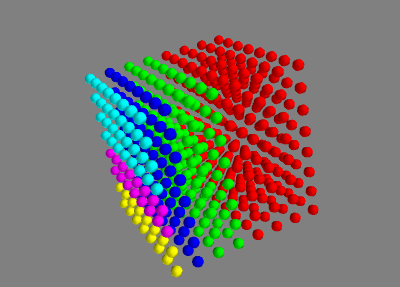
\includegraphics[height=1.2in]{figs/goodallocation}
        \caption{Contiguous}
        \label{fig:overview_sub1}
    \end{subfigure}%
    \hspace{1em}%
    \begin{subfigure}[t]{0.2\textwidth}
        \centering
        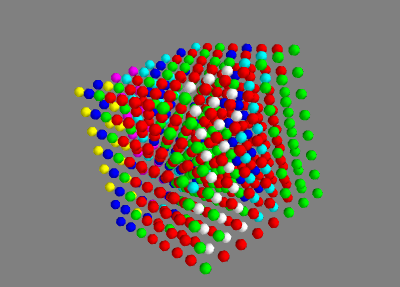
\includegraphics[height=1.2in]{figs/badallocation}
        \caption{Non-contiguous}
        \label{fig:overview_sub2}
    \end{subfigure}%
   \caption{Indication of multiple jobs running concurrently with different allocations. Each job is represented by a specific color. a) shows the effect of partition-based allocation, which reduce the inter-job interference. b) shows non-contiguous allocation, which introduces both intra and inter-job interferences. }
   \label{fig: overview}
\end{figure}

%\begin{figure}[h!] 
%  \centering
%  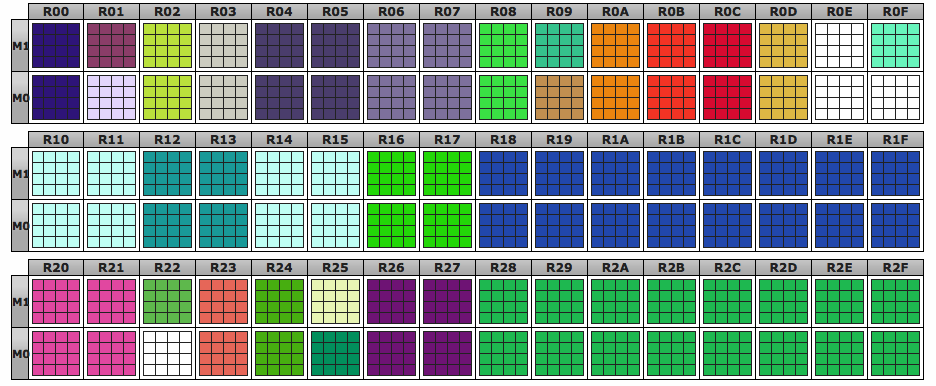
\includegraphics[width=0.38\textwidth]{figs/mira}
%   \caption{The activity of Mira, IBM BlueGene/Q system at Argonne National Lab. Many jobs runninng concurrently on the system. Different jobs represented by specific colors. }
%   \label{fig: mira activity}
%\end{figure}

One of the most prominent  problems is network contention among concurrently running jobs. The network sharing among concurrently running jobs causes communication variability that results in jobs running slower \cite{abhinav-sc13}. The delay of running jobs increases the queueing time of the following submitted jobs, thus leading to low system throughput and utilization \cite{jose-ipdps15}. 

This adverse effect of network sharing can be mitigated by providing jobs with isolated allocations and exclusive network resource. The batch scheduler is responsible for assigning job the amount of nodes it requires. On the widely used torus-connected HPC systems \cite{bgq}\cite{tofu}\cite{titan}, two allocation strategies are commonly used. In the partition based allocation, used in Blue Gene series systems, he scheduler assigns each user job a compact and contiguous set of computing nodes. This strategy favors application performance by providing application with isolated partitions and exclusive network connections, thus reducing network contention caused by concurrently running jobs. However, this strategy can cause internal fragmentation (when more nodes are allocated to a job than it requests) and external fragmentation (when sufficient nodes are available for a request, but they can not be allocated contiguously), therefore leading to lower system utilization that is otherwise possible. The other strategy is non-contiguous allocation, used by Cray XT/XE series, in which free nodes are assigned to user jobs whether they are contiguous or not. Non-contiguous allocation eliminates internal and external fragmentation as seen in partition-based systems, thereby leading to high system utilization. However, it introduces other problems, for example scattering application processes all over the system, causing both inter-job and intra-job contention. The non-contiguous node allocation can significantly reduce job performance, especially for communication-intensive jobs.

%\textcolor{red}{
%Partition-based allocation achieves good job performance by sacrificing system utilization, whereas non-contiguous allocation can result in better system utilization but could severely degrade performance of user jobs. What is needed is a more flexible strategy that provides allocations that minimize intra/inter-job contention but allow greater system utilization. In this work, we propose a guideline for future batch scheduling systems, a smart way to allocate resources with the awareness of jobs communication patterns.
%
%Most existing batch schedulers take so few initiative because it been hold under the obscurantism policy. Whether it use partition-based or non-contiguous policy, means it chooses the benefit of either system or job over the other. Some propose compromised policies like buddy system\cite{buddy system paper} still make the allocation for job blindly without knowing job's communication information. 
%
%Although HPC applications complexity continue to grow, people could get more knowledge about the applications communication information with the help from various parallel application profiling tools, such as TAU\cite{tau}, MPIP\cite{mpip} and DUMPI\cite{sst}. Job's communication trace and performance analysis can be get by using such tool at runtime. 
%
%The off-line study of job's communication traces could be helpful to develop better allocation policies for batch scheduler to make on-line scheduling/allocating decisions. This is because the communication pattern of parallel applications on HPC system can be summarized into a couple of categories\cite{hpdc2015-ornl}. The deep understanding of one application can be helpful to all other applications that conforms to the same communication pattern. Job's communication traces study would be extreme helpful to leadership computing facility too. The set of applications running on those leadership computing facilities is usually stable, and the workloads from those HPC systems is usually has great repetitiveness. We analyzed the workload on Mira, an IBM Blue/Gene Q system at Argonne Leadership Computing Facility, found that most jobs require 2k nodes and about 14 particular jobs consist of the majority its workload\ref{fig: repetitiveness of Mira}. In other word, Mira accommodates mostly some particular 14 jobs and most jobs have the same size.
%}


%=========come back and work from here=============
Rather than choosing blindly between partition-based or non-contiguous allocation, the new allocation strategy choses resources based on a job's communication pattern. With detail analysis of application's communication patterns, our proposed allocation strategy obtains a clear view as to which processes are tightly connected and conduct intensive communication. The ``neighborhood communication" consists of such tightly coupled processes should get a compact allocation. Then, the allocation strategy only needs to guarantee the locality of the subset of the nodes where those ``neighborhood communication" would reside.

In this work, we study the impact of different allocation strategies on intra/inter-job interference on Torus network. Torus networks have been extensively used in the current generation of supercomputers because of their linear scaling on per-node cost and competitive communication performance. On the recent Top500 list, 6 of the top 10 supercomputers use a high-radix torus-interconnected network \cite{top500}. The current generation of IBM Blue Gene/Q (BG/Q) supercomputer, such as Mira at Argonne Nation Laboratory and Sequoia at  Lawrence Livermore National Laboratory, has its nodes connected in a 5D torus network \cite{bgq}. The K computer from Japan uses the “Tofu” system, which is a 6D mesh/torus topology \cite{tofu}. Titan, a Cray XK7 supercomputer located at the Oak Ridge Leadership Computing Facility (OLCF), has nodes connected in a 3D torus within the compute partition \cite{titan}. Although the analysis are based on torus network, the idea conveyed from this work is applicable to networks with different topologies. 

We selected three signature applications from DOE Design Forward Project\cite{design forward webpage} as examples to conduct detailed study about their communication patterns. We use a sophisticated simulation toolkit named CODES, Co-Design of Multi-layer Exascale Storage Architecture\cite{Jason-2011}, from Argonne National Laboratory as a research vehicle to evaluate the performance of our communication pattern aware allocation policy on torus networks. We analyze each application's performance running on torus networks with different dimensionality and interconnected bandwidth. Then, we extend CODES with a Job Mapping API that supports different allocation policies on torus network. Different allocation strategies on torus network are studied with the help of this new Job Mapping API. We analyze the intra/inter-job interference by simulating those three applications running exclusively or concurrently on torus network with different allocation strategies. According to results of our comprehensive exploration, making allocation with consideration about job's communication pattern is a very promising allocation strategy. We believe the idea presented in this work would be the guideline for the design of future HPC batch job scheduler and resource management module. 

The rest of this paper organized as follows. Section \ref{sec:application study} gives a detailed study of the three applications from DOE Design Forward Project. Section \ref{sec:codes} talks about CODEs as research vehicle for our work. Section \ref{sec:config study} shows the performance analysis of three applications on different torus networks. Section \ref{sec:interference} provides detailed analysis about the intra/inter-job interference between three applications on torus network. Section \ref{sec:discussion} talks about the idea of smart allocation strategy with job communication pattern awareness. Section \ref{sec:related_work} talks about the related work in the area and conclusion will be presented in Section \ref{sec:conclusion}. 




\section{Application Study}
\label{sec:application study}

%A parallel application usually conforms to a combination of several basic communication patterns\cite{hpdc2015-ornl}. At its different execution phases, the application's communication behavior may follow different basic patterns respectively. \textcolor{blue}{When we look into the data flow during application execution, most parallel applications start with broadcast operation to distribute the data from root process to other processes\textcolor{red}{ref needed here}, followed by a series of computation and communication that conforms to certain pattern, which is usually the dominant part of application's execution. Before the application come to completion, all the working process will return their results to the root directly or hierarchically.} Parallel application's communication pattern usually involves lots of factors, such as communication intensity, operation-to-operation dependencies and the ``critical path" in its communication topology graph, etc. In this work, we focus on the locality of application's rank-to-rank communication topology graph.

A parallel application usually conforms to a combination of several basic communication patterns\cite{hpdc2015-ornl}. At its different execution phases, the application's communication behavior may follow different basic patterns respectively. Collective communication is often used for data distribution and collection among processes. Nearest Neighbor communication is commonly seen in lots of structured and unstructured mesh physics packages. There are many profiling tools available to capture communication patterns from parallel applications, such as Tuning and Analysis Utilities(TAU)\cite{tau}, mpiP\cite{mpip}. They can help analysis parallel application, providing information like the percentage of different MPI operations of the applications, communication topology, the amount data transferred between processes.

In this work, we provide detailed analysis about the communication pattern of three DOE MiniApps. MiniApps are reduced proxy applications that encapsulate the salient performance of larger full size applications\cite{miniapp}. Since we only focus on the dominant communication pattern of parallel applications, these MiniApps are perfect candidates for analysis the application's performance on different allocations or on new network architectures. We choose three MiniApps, namely, Algebraic Multigrid Solver(AMG), Geometric MultiGrid(MultiGrid) and CrystalRouter. Their representative communication patterns that are commonly seen in the HPC system workload. The communication pattern figures we present here are generated with the IPM\cite{ipm} data from \cite{design forward webpage}.


\subsection{AMG}
\label{sec:amg}


\begin{figure}[t!]
    \centering
    \begin{subfigure}[t]{0.22\textwidth}
        \centering
        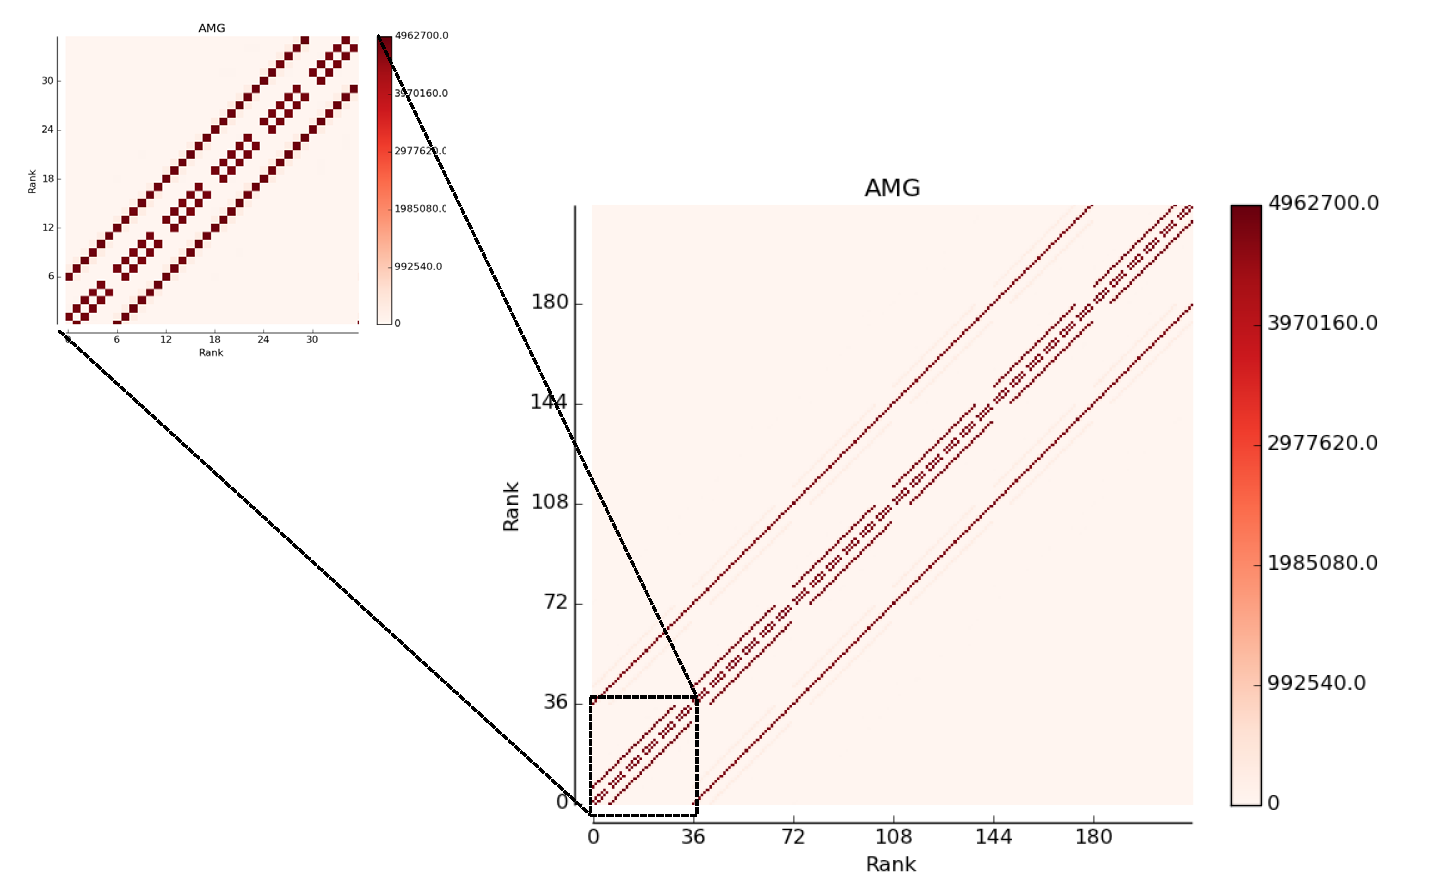
\includegraphics[height=1.2in]{figs/appstudy/amg/amg_pip}
        \caption{Communication Topology}
        \label{fig: amg communication topology}
    \end{subfigure}%
    ~
    \begin{subfigure}[t]{0.22\textwidth}
        \centering
        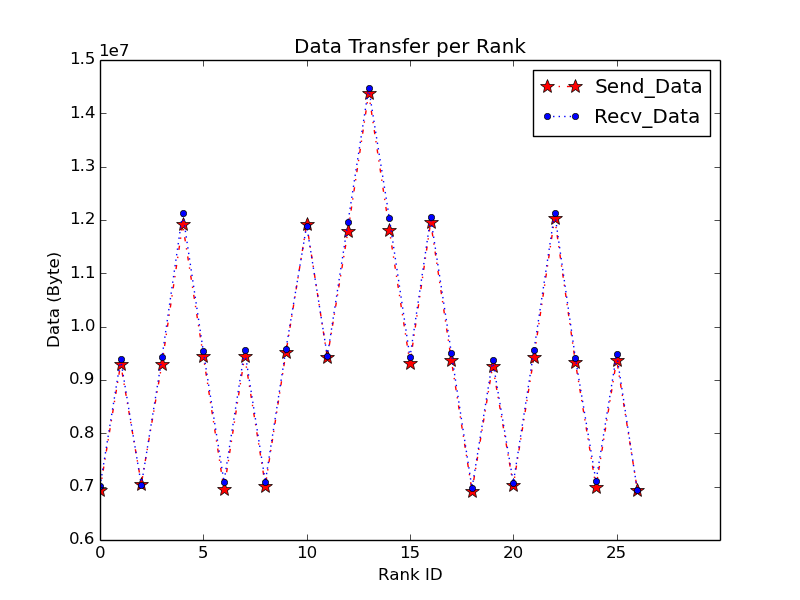
\includegraphics[height=1.2in]{figs/appstudy/amg/amg_data_transfer}
        \caption{Data Volume}
        \label{fig: amg data trans}
    \end{subfigure}
    \caption{AMG. (a) rank-to-rank communication topology graph. (b) the data sent/received by each rank in AMG.}
\end{figure}

AMG is the MiniApp of Algebraic Multigrid Solver, which is a parallel algebraic multigrid solver for linear systems arising from problems on unstructured mesh physics packages. It has been derived directly from the BoomerAMG solver that is being developed in the Center for Applied Scientific Computing (CASC) at LLNL\cite{amg}. The dominant communication pattern is this regional communication with decreasing message size for different parts of the multigrid v-cycle.

Figure \ref{fig: amg communication topology} shows the communication topology of a small scale AMG with 27 MPI Ranks. Here we prefer to show the communication topology with small scale version of the MiniApp because the dominant communication pattern of the application doesn't change with its scale. We can make the observation from the upper-left of the figure that each rank in AMG has intense communication between 3 other ranks, such as rank 0 between rank 1, 3 and 9, rank 1 between 2, 4 and 10, etc. And this relation is also symmetric along the main diagnal. The dominant communication pattern is quite obvious when we identify this relation between ranks.

Figure \ref{fig: amg data trans} shows the amount of data each rank transferred in AMG. The blue line shows that total data amount transferred from each rank, while the red shows the amount of received data and green shows the amount of send data. The first thing we can spot from the figure is that for each rank, the amount of data sent and received are basically the same, which also well explain the symmetry of the application's dominant communication pattern. And the second thing we can find about AMG is that the data transfer amount also has a symmetric pattern. Rank 0 has the same amount of data transfer as Rank 26, Rank 1 as of Rank 25, etc.

AMG represents a group of applications whose dominant communication pattern is Nearest Neighbor. Applications with such similar dominant communication pattern are like PARTISN, SNAP\cite{design forward webpage}.


\subsection{Crystal Router}
\label{sec:crystalrouter}

\begin{figure}[t!]
    \centering
    \begin{subfigure}[t]{0.22\textwidth}
        \centering
        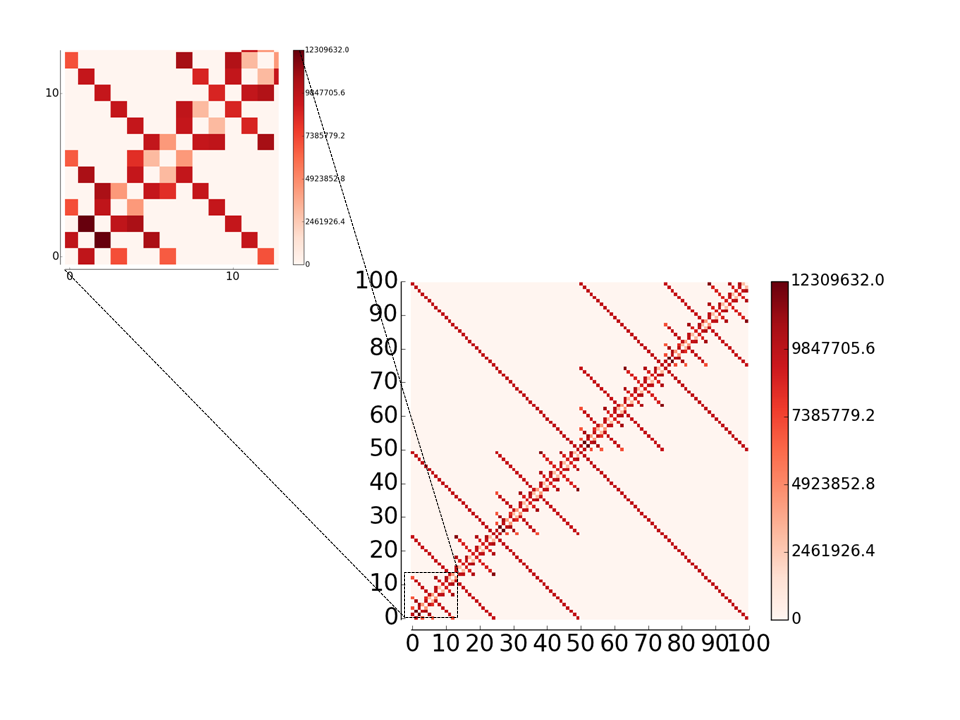
\includegraphics[height=1.2in]{figs/appstudy/cr/cr_pip}
        \caption{Communication Topology}
        \label{fig: cr communication topology}
    \end{subfigure}
    ~
    \begin{subfigure}[t]{0.22\textwidth}
        \centering
        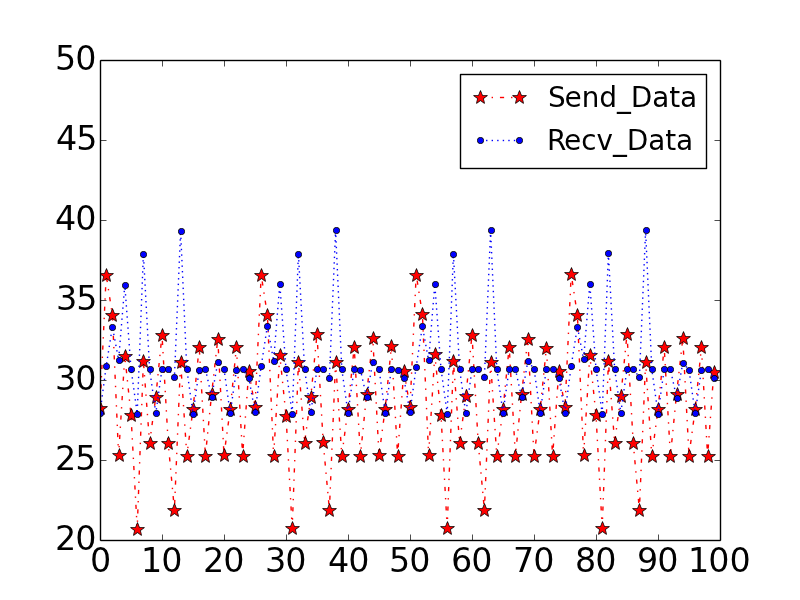
\includegraphics[height=1.2in]{figs/appstudy/cr/cr_data_transfer}
        \caption{Data Volume}
        \label{fig: cr data trans}
    \end{subfigure}
    \caption{CrystalRouter. (a) rank-to-rank communication topology graph. (b) the data sent/received by each rank in CrystalRouter. }
\end{figure}

The second MiniApp we have is Crystal Router, which is the extracted communication kernel of the full application Nek5000. Nek5000\cite{crystalrouter} is a spectral element CFD application developed at Argonne National Laboratory. It features spectral element multigrid solvers coupled with a highly scalable, parallel coarse-grid solver that widely used for projects including ocean current modeling, thermal hydraulics of reactor cores, and spatiotemporal chaos. The communication kernel of Nek5000, CrystalRouter demonstrates the "many-to-many" communication pattern through scalable multi-stage communication process. \textcolor{yellow}{The way CrystalRouter works is nodes compute for a while, then synchronize and communicate, continually alternating between these two types of activities.}

As we can see from Figure \ref{fig: cr communication topology}, every 5-rank is a compact community, where data transfer is very intensive. Beside the "5-rank community", there is "pair-wise" global data transfer in CrystalRouter. Obviously, there is data transfer alone the diagnal. \textcolor{yellow}{This is because messages would be buffered on their node of origin until a synchronization point was reached when a single system call sent every message to its destination in one pass.} When the scale of Crystal Router increase to 100, the "5-rank community" is still the dominant pattern in a hierarchical manner. The same pattern can be observed from the global data transfer. Our observation about the dominant communication pattern of CrystalRouter is the multi-stage "5-rank community" and "pair-wise" global data transfer happen hierarchically as the scale of the application increase.

Figure \ref{fig: cr data trans} shows the amount of data each rank transferred in Crystal Router. The locality pattern of "5-rank community" can still be spotted in this figure. The spiky shape occurs in the frequency of every 5 rank. Unlike AMG, the there is variance between the amount of data send and received for each rank. This is due to the specific feature of Crystal Router's communication pattern.

CrystalRouter represents a group of applications whose dominant communication is a hybrid of multi-stage local and hierarchical global communication.



\subsection{MultiGrid}
\label{sec:multigrid}
Different from AMG, MultiGrid is geometric multigrid v-cycle from production elliptic solver BoxLib, a software framework for massively parallel block-structured adaptive mesh refinement (AMR) codes. MultiGrid conforms to Many-to-Many communication pattern with decreasing message size and collectives for different parts of the multigrid v-cycle. It is widely used for structured grid physics packages. Figure\ref{fig: mg communication topology} shows the communication topology of MultiGrid and Figure\ref{fig: mg data trans} shows the the amount of data transferred between ranks in MultiGrid.

\begin{figure}[t!]
    \centering
    \begin{subfigure}[t]{0.22\textwidth}
        \centering
        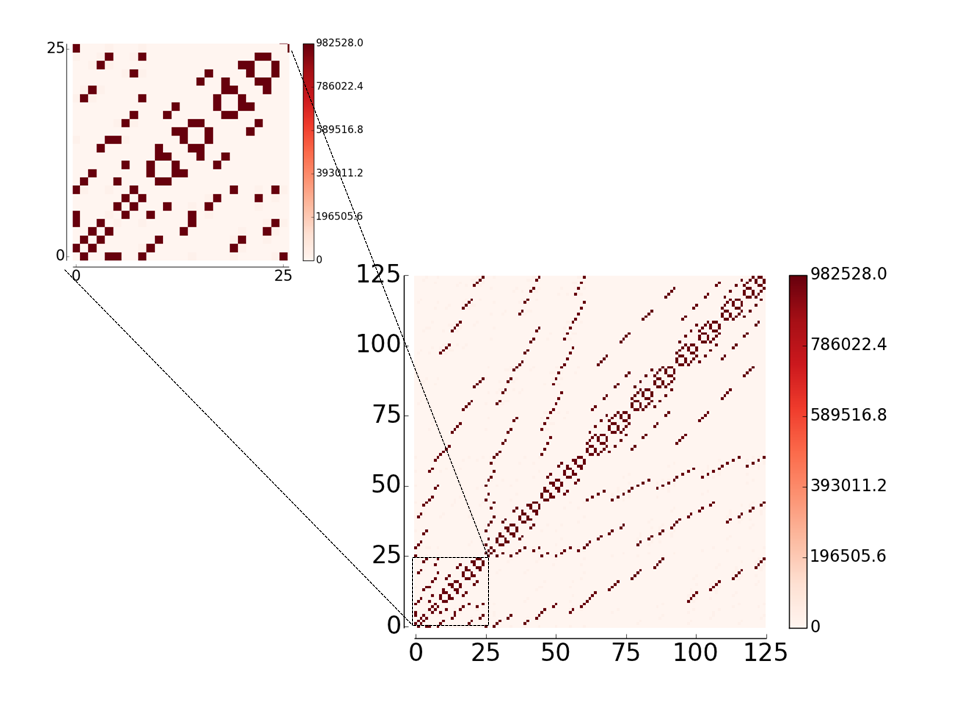
\includegraphics[height=1.2in]{figs/appstudy/mg/mg_pip}
        \caption{Communication Topology}
        \label{fig: mg communication topology}
    \end{subfigure}
    ~
    \begin{subfigure}[t]{0.22\textwidth}
        \centering
        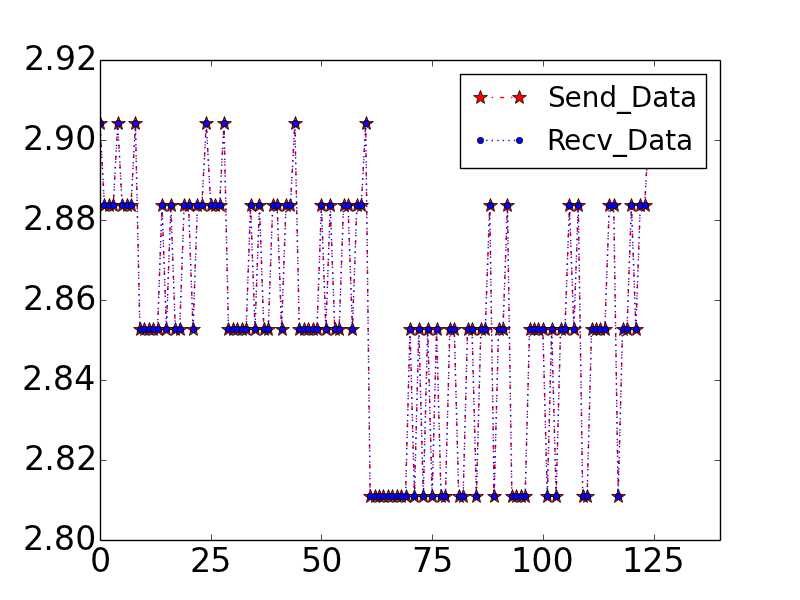
\includegraphics[height=1.2in]{figs/appstudy/mg/mg_data_transfer}
        \caption{Data Volume}
        \label{fig: mg data trans}
    \end{subfigure}
    \caption{MultiGrid. (a) rank-to-rank communication topology graph. (b) the data sent/received by each rank in MultiGrid.}
\end{figure}


MultiGrid represents a group of applications whose dominant communication pattern is Many-to-Many (some literatures also refer it as All-to-All \cite{hpdc2015-ornl}).  




%\begin{figure*}[t!]
%    \centering
%    \begin{subfigure}[t]{0.32\textwidth}
%        \centering
%        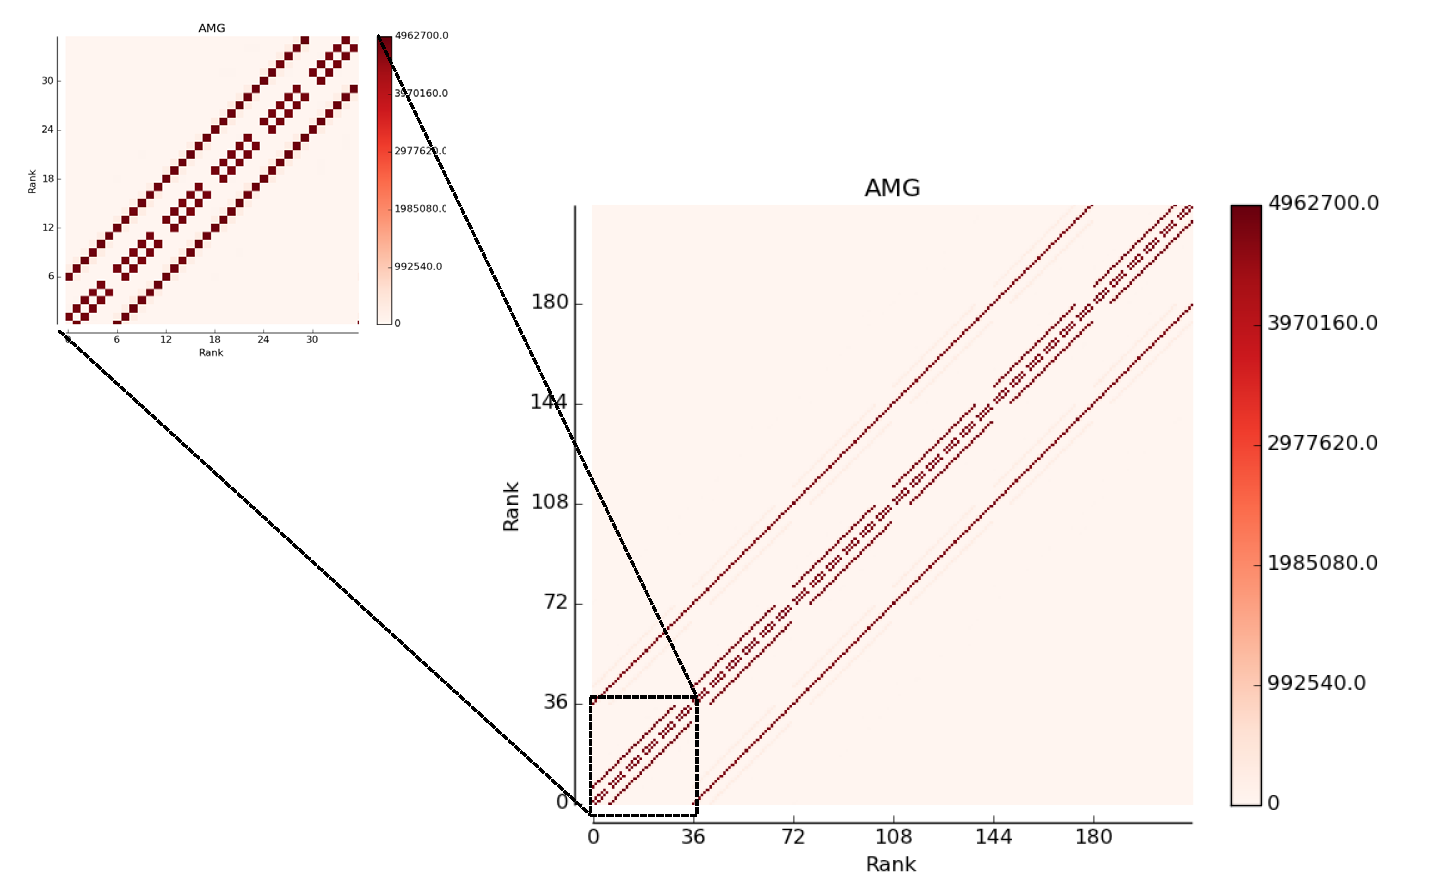
\includegraphics[height=1.2in]{figs/appstudy/amg/amg_pip}
%        \caption{AMG}
%        \label{fig: amg communication topology}
%    \end{subfigure}%
%    ~ 
%    \begin{subfigure}[t]{0.32\textwidth}
%        \centering
%        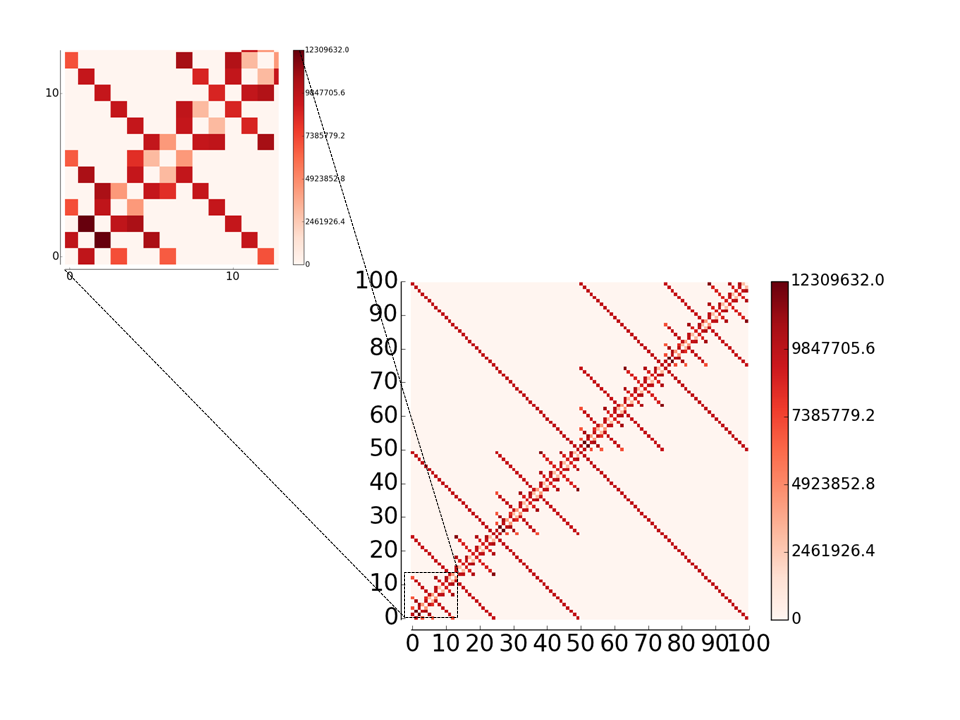
\includegraphics[height=1.2in]{figs/appstudy/cr/cr_pip}
%        \caption{CrystalRouter}
%        \label{fig: cr communication topology}
%    \end{subfigure}
%    ~
%    \begin{subfigure}[t]{0.32\textwidth}
%        \centering
%        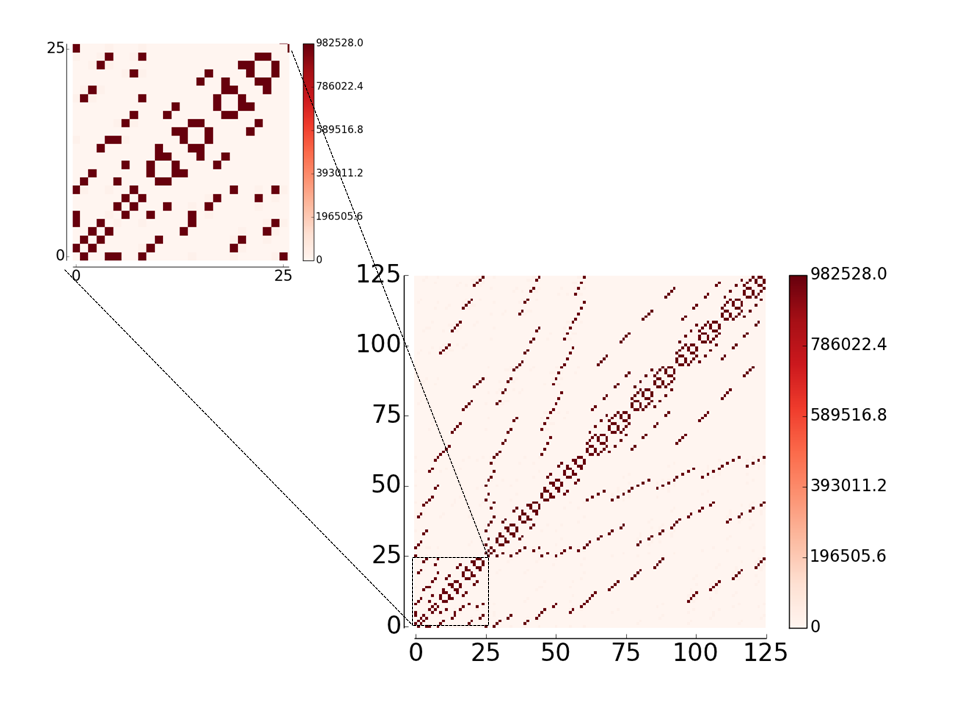
\includegraphics[height=1.2in]{figs/appstudy/mg/mg_pip}
%        \caption{MultiGrid}
%        \label{fig: mg communication topology}
%    \end{subfigure}
%    \caption{Caption place holder}
%\end{figure*}
%
%\begin{figure*}[t!]
%    \centering
%    \begin{subfigure}[t]{0.32\textwidth}
%        \centering
%        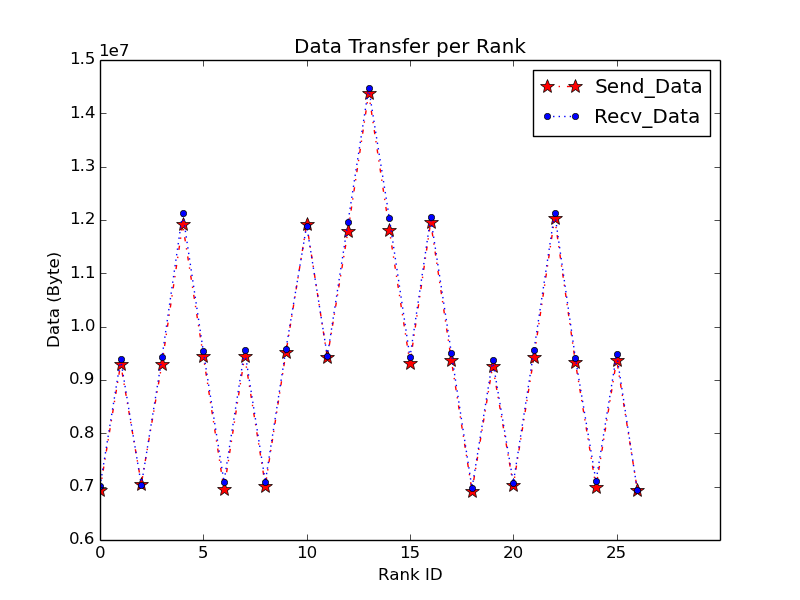
\includegraphics[height=1.2in]{figs/appstudy/amg/amg_data_transfer}
%        \caption{AMG DATA}
%        \label{fig: amg data trans}
%    \end{subfigure}
%    ~
%    \begin{subfigure}[t]{0.32\textwidth}
%        \centering
%        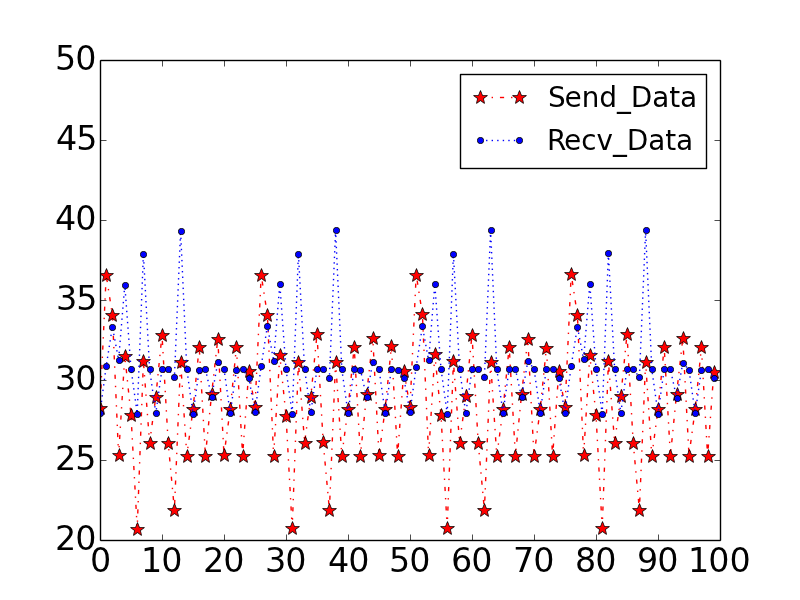
\includegraphics[height=1.2in]{figs/appstudy/cr/cr_data_transfer}
%        \caption{CR DATA}
%        \label{fig: cr data trans}
%    \end{subfigure}
%    ~
%    \begin{subfigure}[t]{0.32\textwidth}
%        \centering
%        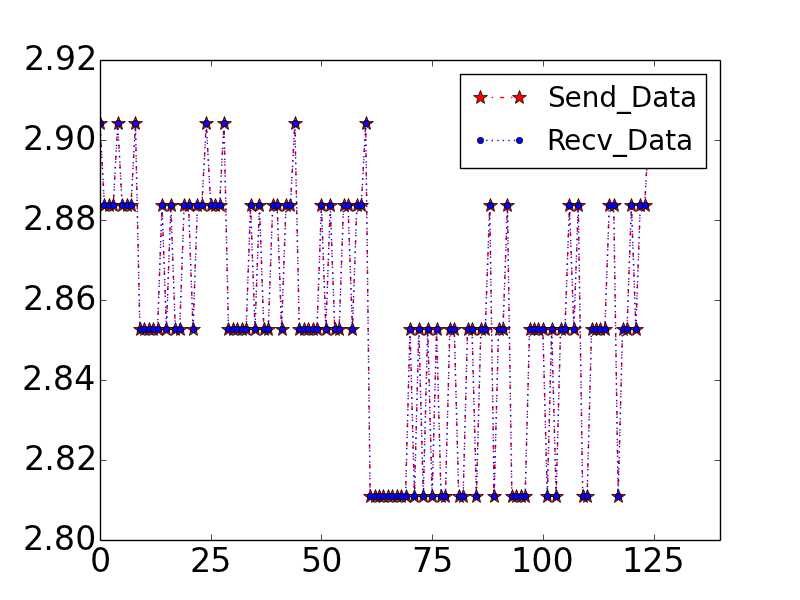
\includegraphics[height=1.2in]{figs/appstudy/mg/mg_data_transfer}
%        \caption{MG DATA}
%        \label{fig: mg data trans}
%    \end{subfigure}
%    \caption{Caption place holder}
%\end{figure*}


%We summarize the benchmarks and MiniApps on DOE design forward webpage\cite{design forward webpage}, as shown in Table \ref{tab: app summary}. According to their dominant communication patterns, there are three categories, namely Nearest Neighbor, All-to-All and 3D Lattice. The three applications studies in this work are representative for different categories. 


%\begin{table}[ht]
%\begin{center}
%\caption{ Summary of dominant communication pattern of MiniApps from DOE design forward project.} 
%\label{tab: app summary}
%\begin{tabular}{l c c c c} 
%\toprule % Top horizontal line
%\toprule
%\multicolumn{2}{c}{Applications} \\
%%\cmidrule(l){2-3}
%\textbf{Dominant CP}  &  &  & &\\ % Column names row
%\midrule % In-table horizontal line
%\textbf{Nearest Neighbor}   &AMG    & SNAP  & PARTISN &\\ % Content row 1
%
%\midrule
%\textbf{All-to-All}  &CrystalRouter    &BoxLib AMR    &MiniFE\\ % Content row 1
%
%\midrule
%\textbf{3D Lattice}   &MultiGrid    & MiniDFT    &FillBoundary \\ % Content row 1
%       
%\midrule
%\bottomrule % Bottom horizontal line
%\end{tabular}
%\end{center}
%\end{table}

%\textcolor{red}{Apps Summary} These three applications have representative communication patterns that are commonly seen in the HPC system workload. AMG represents a group of applications whose dominant communication pattern is Nearest Neighbor. MultiGrid represents applications whose dominant communication pattern is Many-to-Many (some literatures also refer it to All-to-All\cite{hpdc2015-ornl}). CrystalRouter represents those applications whose dominant communication is a hybrid of multi-stage local communication and hierarchical global communication. 





\section{Research Vehicle}
\label{sec:codes}

It is impossible to accurately study the interference between concurrently running jobs with different allocation strategies on production systems. There are a couple of reasons for that. First, the allocation strategy used on production machine is part of the system software, which can not be changed by user. Even the system administrator is not authorized to make that change. Second, it is unrealistic to reserve the system exclusively to run the same job with desired allocation without interference then compare the results to that in the presence of interference. Due to those reasons, we resort to simulation for this work.

There are couple of simulation platform to study the behavior of large scale systems. SimGrid from Inria is a versatile simulation tool sets that provide simulation for Grids, Clouds and HPC systems\cite{simgrid}. The Structural Simulation Toolkit (SST) from Sandia National Lab was developed to explore innovations in highly concurrent systems where the ISA, microarchitecture, and memory interact with the programming model and communications system\cite{sst}.

A simulation toolkit named CODES (Co-Design of Multi-layer Exascale Storage Architecture) from Argonne National Lab enables the exploration of simulating different HPC networks with high fidelity\cite{Jason-2011}\cite{mubarak-sc2012}. CODES is built on top of Rensselaer Optimistic Simulation System (ROSS) parallel discrete-event simulator, which is capable of processing billions of events per second on leadership-class supercomputers\cite{ross}. CODES support both torus and dragonfly network with high fidelity flit-level simulation. In this work, we only use torus network to show the impact of node allocation to job with different dominant communication patterns. CODES has this network workload component that capable of conducting trace-driven simulation. It can take real MPI application trace generated by SST DUMPI\cite{sst} to drive CODES network models. We implemented a Job Mapping API for CODES, which can provide flexible job allocation strategies. The new API can help us to explore the impact of different allocation strategies to those three applications in Section \ref{sec:application study}


\section{Experiment}
\label{sec:experiment results}

CODES can provide Torus network model with good scalability and high fidelity\cite{codes-torus}. In this section, we will first study the communication behavior of three applications on torus network with different dimensionality and bandwidth configurations. Then, we study the intra- and inter-job interference with these three applications by running them exclusively and concurrently with different allocation strategies. 

\subsection{Configuration Study }
\label{sec:config study}

The topology of torus network is k-ary n-cube, with $k^n$ nodes in total arranged in an n-dimensional grid having k nodes in each dimension. Each node has 2$\times$ n direct linked neighbor nodes. The torus network performance is determined by its dimensionality and link bandwidth. As the increase of the dimensionality of torus network, so does the number of links connected with each node. The increased aggregated bandwidth of each node will definitely reduce the data transfer time of each rank in the application. Figure \ref{fig:dimensionality-study} shows the performance of the AMG, CrystalRouter and MultiGrid on a 2K node torus network model with a 3D torus (16x16x8), a 5D torus (8x4x4x4x4), and a 7D torus (4x4x4x4x2x2x2). The bandwidth of direct link between nodes is 2GiB/s in each direction, thus, the aggregated bandwidth is 12GiB/s per node in 3D torus, 20GiB/s per node in 5D torus, and 28GiB/s per node in 7D torus.

 
We can see from Figure \ref{fig:dimensionality-study} that the data transfer time of those three applications are greatly reduced as the dimensionality increases. The increased aggregated bandwidth of each node can accelerate the transfer of data. This can justify the fidelity and consistency of the torus network model. We allocate each rank within each application linearly on the 3D torus. However, due to the variance of data transfer volume of each rank, AMG's data transfer time has great dispersion, shown as the outliers above the boxes in Figure \ref{fig:dimen-amg}. There is no such great dispersion for CrystalRouter and MultiGrid, shown in Figure \ref{fig:dimen-cr} and \ref{fig:dimen-mg}, since no great variance of data transfer amount of each rank in these applications.

\begin{figure*}[t!]
    \centering
    \begin{subfigure}[t]{0.32\textwidth}
        \centering
        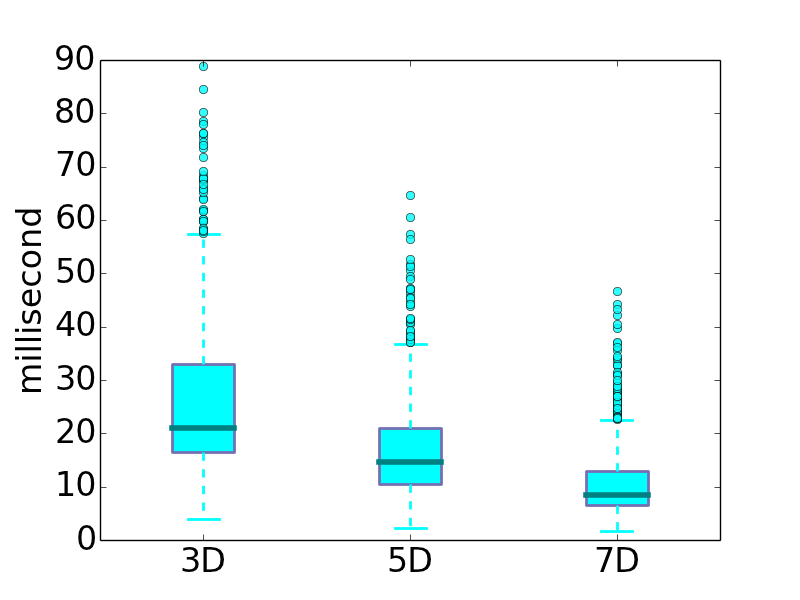
\includegraphics[height=1.5in]{figs/dimenstudy/amg_box}
        \caption{AMG}
        \label{fig:dimen-amg}
    \end{subfigure}%
    \hspace{1em}%
    \begin{subfigure}[t]{0.32\textwidth}
        \centering
        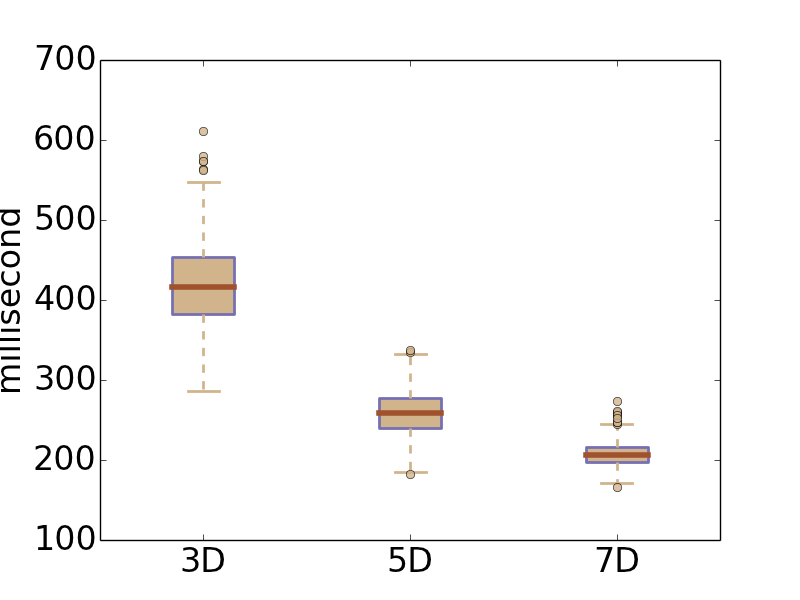
\includegraphics[height=1.5in]{figs/dimenstudy/cr_box}
        \caption{CrystalRouter}
        \label{fig:dimen-cr}
    \end{subfigure}%
    \begin{subfigure}[t]{0.32\textwidth}
        \centering
        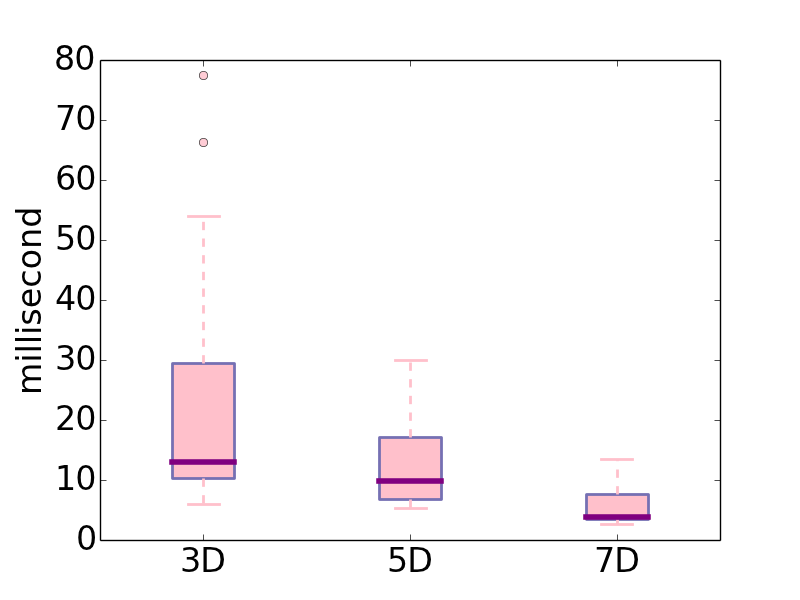
\includegraphics[height=1.5in]{figs/dimenstudy/mg_box}
        \caption{MultiGrid}
        \label{fig:dimen-mg}
    \end{subfigure}%
   \caption{Data Transfer Time of AMG, CrystalRouter and MultiGrid on 3D, 5D and 7D torus network. The network bandwidth increases as the dimensionality grows. Due to the data volume sent/received by each rank greatly varies, there is great dispersion of AMG's data transfer time, shown as outliers above the boxes in Figure \ref{fig:dimen-amg}.}
   \label{fig:dimensionality-study}
\end{figure*}


Then we use fixed dimensionality to study the impact of increased bandwidth. We run these three applications on 5D torus with direct link bandwidth increases from 2GiB/s, to 4GiB/s and 8GiB/s. As shown in Figure \ref{fig:bandwidth-study}, the data transfer time of each application can be greatly reduced as the bandwidth increases. 

\begin{figure*}[t!]
    \centering
    \begin{subfigure}[t]{0.32\textwidth}
        \centering
        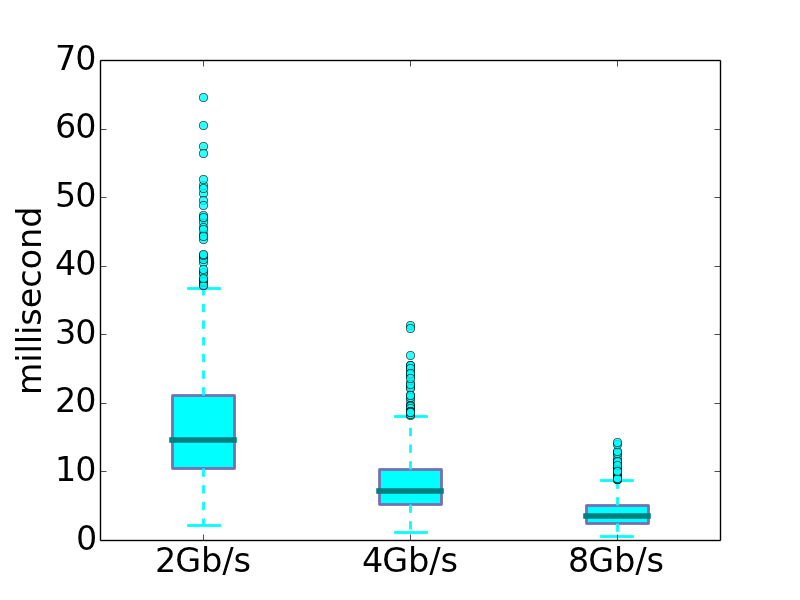
\includegraphics[height=1.5in]{figs/bandwidthstudy/amg_bw_box}
        \caption{AMG}
        \label{fig:bdwstudy-amg}
    \end{subfigure}%
    \hspace{1em}%
    \begin{subfigure}[t]{0.32\textwidth}
        \centering
        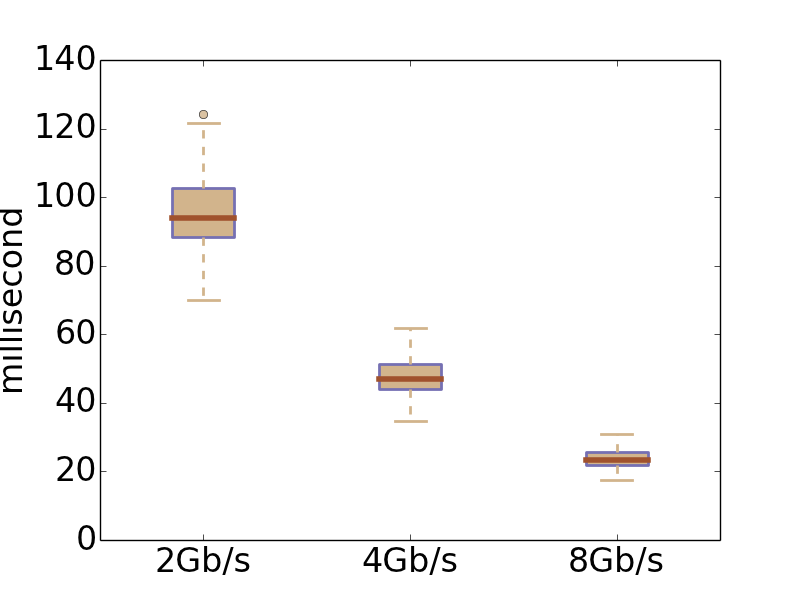
\includegraphics[height=1.5in]{figs/bandwidthstudy/cr_bw_box}
        \caption{CrystalRouter}
        \label{fig:bdwstudy-cr}
    \end{subfigure}%
    \begin{subfigure}[t]{0.32\textwidth}
        \centering
        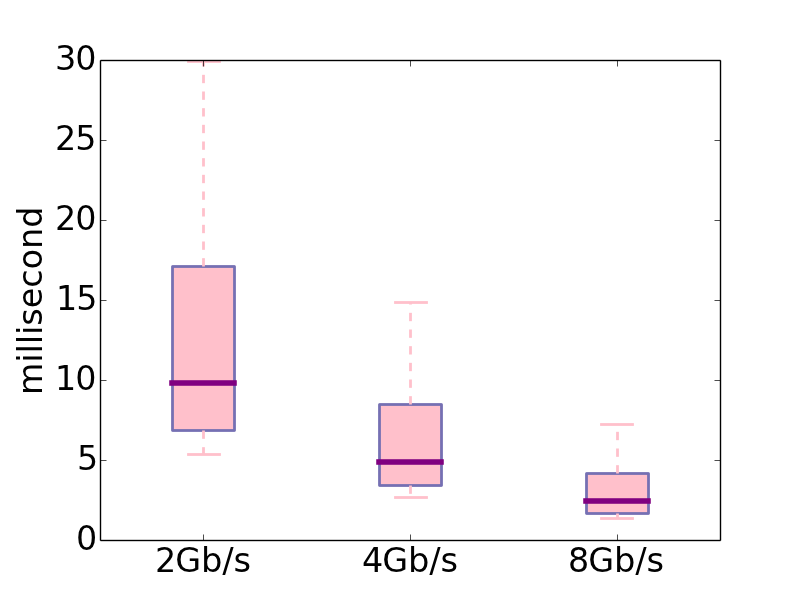
\includegraphics[height=1.5in]{figs/bandwidthstudy/mg_bw_box}
        \caption{MultiGrid}
        \label{fig:bdwstudy-mg}
    \end{subfigure}%
   \caption{Data transfer time of AMG, CrystalRouter and MultiGrid on 5D torus network with 2Gb/s, 4Gb/s and 8Gb/s direct link bandwidth. }
   \label{fig:bandwidth-study}
\end{figure*}

We also study the impact of dimensionality with fixed aggregated bandwidth. We use 3D, 5D and 7D torus network with the same per-node aggregated bandwidth, which is 28Gb/s. With the same aggregated bandwidth, higher dimensionality means shorter diameter and pair-wise distance between nodes. The bandwidth between nodes in each torus network are shown in Table \ref{tab: fix-bandwidth}

\begin{table}[ht]
\begin{center}
\caption{Torus networks with same aggregated bandwidth} 
\label{tab: fix-bandwidth}
\begin{tabular}{l c c c} 
\toprule % Top horizontal line
\toprule
&\multicolumn{3}{c}{Bandwidth } \\
\cmidrule(l){2-4}
Dimension  & direct & aggregate &\\ % Column names row
\midrule % In-table horizontal line
3D      & 4.67Gb/s  & 28Gb/s  & \\  % Content row 1
\midrule % In-table horizontal line
5D    & 2.8Gb/s  & 28Gb/s  &\\ % Content row 1
\midrule % In-table horizontal line
7D    & 2Gb/s & 28Gb/s & \\
\midrule
\bottomrule % Bottom horizontal line
\end{tabular}
\end{center}
\end{table}

As we see from Figure \ref{fig:samebd-amg}, the quartiles of ``3D" box is a little bit higher (1\%) than that of ``5D", which means increasing dimensionality from 3D to 5D has little improvement on the average data transfer time for AMG.  However, there is obvious reduction in those outliers between 3D and 5D. When dimensionality increases up to 7D, the improvement in terms of average data transfer time is still small, but more outliers above the top whisker can be spotted. 

The performance of CrystalRouter actually deteriorate as the torus dimensionality increasing, shown in Figure \ref{fig:samebd-cr}. This is due to the direct link bandwidth reduces from 4.67Gb/s to 2Gb/s, as dimension increases from 3D to 7D. CrystalRouter's large amount of intensive local data transfer benefit more from higher direct link bandwidth than its global transfer from lower diameter and shorter pair-wise distance between nodes. 

The performance of MultiGrid is gradually improved as the dimensionality of torus network increases, shown in Figure \ref{fig:samebd-mg}. The reduced diameter and shorten pair-wise distance between nodes would make the ``Many-to-Many" global data transfer in MultiGrid more efficient. 

We can get the observation that higher dimensionality of torus network would improve the performance of application with ``Many-to-Many" communication patterns, while application with intensive local communication like ``Nearest Neighbor" won't benefit much from higher dimensionality. 

\begin{figure*}[t!]
    \centering
    \begin{subfigure}[t]{0.32\textwidth}
        \centering
        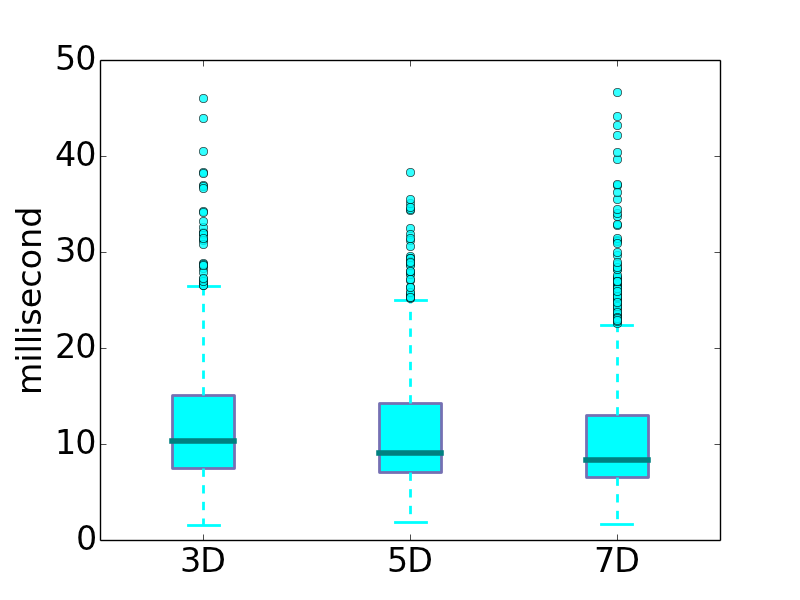
\includegraphics[height=1.5in]{figs/samebdw/amg}
        \caption{AMG}
        \label{fig:samebd-amg}
    \end{subfigure}%
    \hspace{1em}%
    \begin{subfigure}[t]{0.32\textwidth}
        \centering
        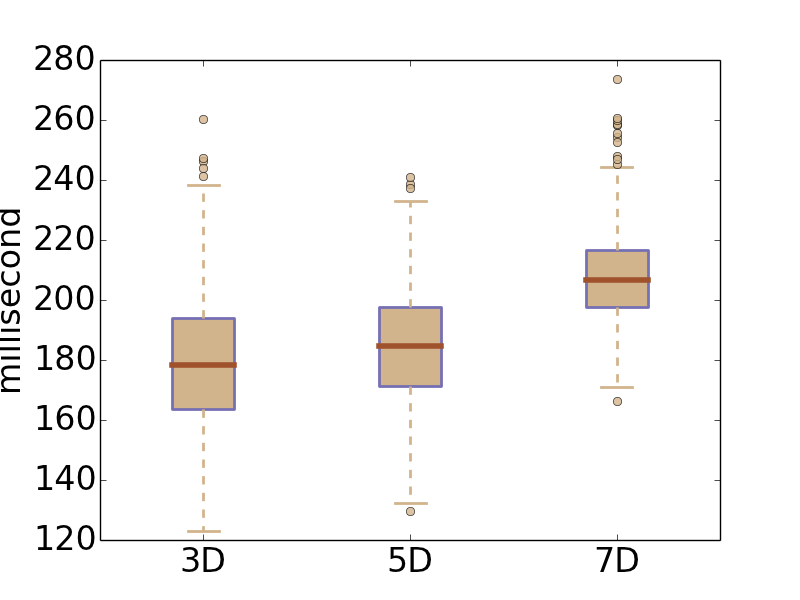
\includegraphics[height=1.5in]{figs/samebdw/cr}
        \caption{CrystalRouter}
        \label{fig:samebd-cr}
    \end{subfigure}%
    \begin{subfigure}[t]{0.32\textwidth}
        \centering
        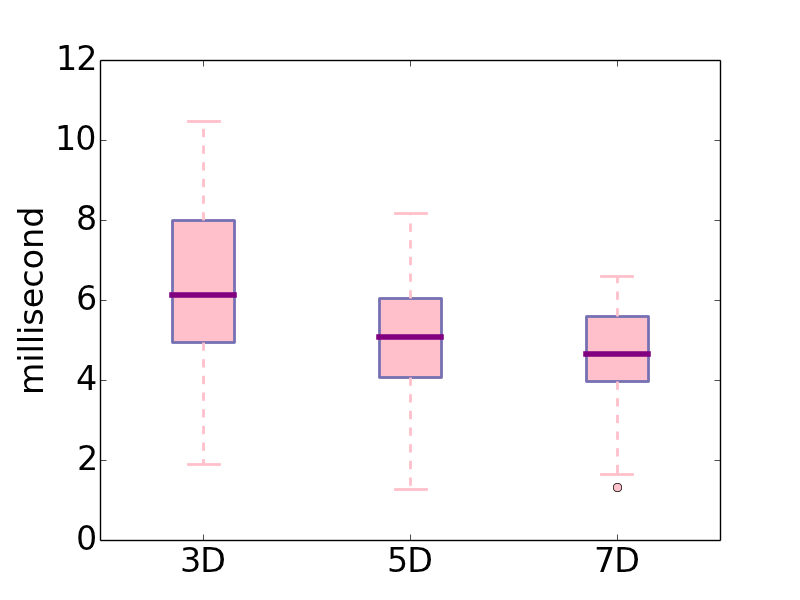
\includegraphics[height=1.5in]{figs/samebdw/mg}
        \caption{MultiGrid}
        \label{fig:samebd-mg}
    \end{subfigure}%
   \caption{Data transfer time of AMG, CrystalRouter and MultiGrid on 3D, 5D and 7D torus network with same aggregated bandwidth. }
   \label{fig: bandwidth-time-box}
\end{figure*}


\subsection{Interference Analysis}
\label{sec:interference}

Communication variability due to network sharing can cause application performance degradation in two ways, namely intra- and inter-job interference. The \textbf{\emph{intra-job interference}} refers to the network contention between ranks within each application. There are lots of research works\cite{jingjin}\cite{ozan} try to come up with better task mapping algorithms to alleviate the intra-job interference, which is out the scope of our work. In this work, we focus on the analysis of such interference with different allocations.

\textbf{\emph{Inter-job interference}} is introduced by concurrently running jobs that adjacent to each other sharing network resources. Such interference has been identified as one of the major culprits for application's performance variability\cite{abhinav-sc13}\cite{skinner}\cite{rosenthal}. Inter-job interference is a more prominent issue for system adopted non-contiguous allocation policy than partition-based system. Application's communication time can vary from 36\% faster to 69\% slower due to inter-job interference when running on non-contiguous allocation\cite{abhinav-sc13}.

In this section we will study both kinds of interference with with AMG, CrystalRouter and MultiGrid in their medium scale. To be specific, we choose AMG with 216 ranks, CrystalRouter with 100 ranks, and MultiGrid 125 ranks and simulate their running on 2K-node (16 $\times$ 16 $\times$ 8) 3D torus network.

We can get observations that 
\begin{enumerate}
    \item The compact allocation can not guarantee the best performance for every application. 
    \item The performance of application conforms to Nearest Neighbor communication pattern keep relatively stable with different shape allocations, while application conforms to ``Many-to-Many" communication pattern prefer compact allocation. 
    \item The allocation unit size should be decided according to application's communication pattern. Unit size that big enough to preserve the locality of the application will result better performance. 
\end{enumerate}


\begin{figure}[t!]
    \centering
    \begin{subfigure}[t]{0.2\textwidth}
        \centering
        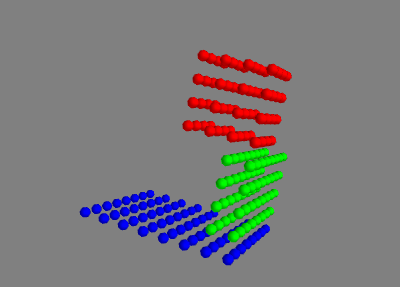
\includegraphics[height=1.2in]{figs/cont/allocation}
        \caption{ }
        \label{fig:cont_sub1}
    \end{subfigure}%
    \hspace{1em}%
    \begin{subfigure}[t]{0.2\textwidth}
        \centering
        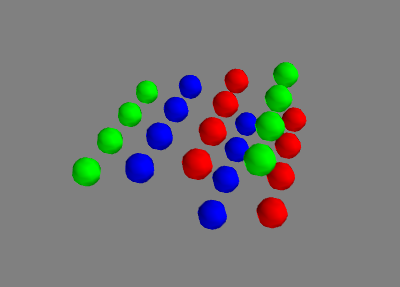
\includegraphics[height=1.2in]{figs/inter-job/noncont/sharing}
        \caption{ }
        \label{fig:noncont_sub1}
    \end{subfigure}%
    \caption{(a) Illustrates the contiguous allocation for 64-node job in three different shapes. ``Blue" is 2D mesh, ``Green" is 3D-unbalanced cube and ``Red" is 3D-balanced cube. (b) Illustrates the non-contiguous allocation. Different colors represent different jobs. The nodes assigned to different jobs are interleaved, the allocation unit is 4-node.}
\end{figure}


\subsubsection{Intra-Job Interference Analysis}
\label{sec: introjob}

To study the intra-job interference of each job, we simulate each job running on 3D torus network with different allocation shapes. We assign each application with three different shapes allocation, i.e. 3D balanced-cube, 3D unbalanced-cube, 2D mesh.

3D balanced-cube, shown as red in Figure \ref{fig:cont_sub1}, can guarantee the minimum \emph{average pair-wise distance} within the allocation. There are some research work like \cite{leung} \cite{abhinav-sc13} try to prove that compact allocation can guarantee job with better performance. They use many metrics to evaluate the compactness of the allocation, such as \emph{average pair-wise distance}, \emph{diameter} and \emph{contiguity}. In this work, we select 3D balanced-cube as the most compact allocation on a 3D torus network. 

3D unbalanced-cube, shown as green in Figure \ref{fig:cont_sub1}, is a rectangular prism, which is the possible allocation shape on system with asymmetric networks. For example, Blue Waters Cray XE6/XK7 system network is 3D torus with Gemini routers. The network connections in the \emph{y}direction have only half the bandwidth of the cables used in the \emph{x} and \emph{z} directions. In order to take advantage of the faster links in the \emph{x} and \emph{z} directions, job allocation is always start from X-Z plane, which leads to a rectangular prism shaped allocation\cite{RF}.

2D mesh, shown as blue in Figure \ref{fig:cont_sub1}, can be cut out from a single layer of the 3D torus. 2D mesh is a very common allocation shape in torus network for both partition-based and non-contiguous allocation strategies. For example, Cray Application Level Placement Scheduler indexes the nodes in torus network into a list and make allocation by simply works off the this list \cite{carl-cug}. When the list is obtained by sorting the nodes based on their spacial coordinates in the torus, allocation made off from this list will be 2D mesh. The IBM Blue/Gene Q supercomputer Mira at Argonne Leadership Computing Facility also allow its allocation partition configured into mesh \cite{zhou-ipdps}. 


There are lots of research work try to design fancy allocation algorithms to provide application with most compact allocation. However, providing cubical allocation without considering application's communication pattern won't guarantee the best performance for every application. Figure \ref{fig:shapstudy-amg} shows that for AMG, who has this symmetric local communication pattern through all ranks, spent less time when assigned with 3D-unbalanced allocation than 3D-balanced. And MultiGrid gets the best performance (shortest data transfer time) when running on 3D-balanced allocation, as shown in Figure \ref{fig:shapstudy-mg}. Since MultiGrid's communication pattern is many-to-many dominant, 3D-balanced is the most compact allocation with shortest pair-wise distance between nodes, which can reduce the aggregated hops for transferring message between ranks in MultiGrid. CrystalRouter has with both dominant local communication and multi-stage global data transfer, the 3D-balance is also the best allocation, but its advantage over 3D-unbalanced is not that obvious as to MultiGrid, as shown in Figure \ref{fig:shapstudy-cr}.

\emph{OBSERVATION}
Compact allocation should be provided to application with global data transfer, such as those conforms to ``Many-to-Many" communication pattern. Application with dominant communication pattern like Nearest Neighbor won't fully utilize the compact allocation and could get even better performance on a relaxed allocation shape. 



\begin{figure*}[t!]
    \centering
    \begin{subfigure}[t]{0.32\textwidth}
        \centering
        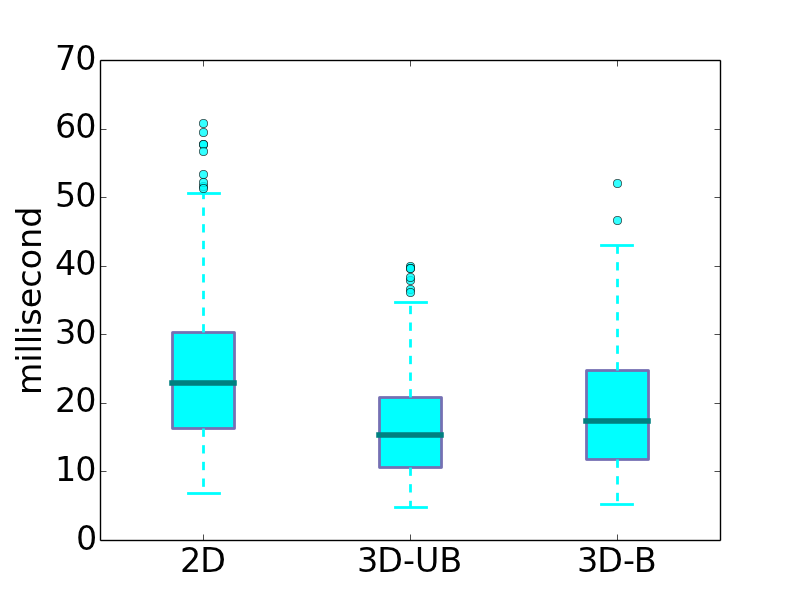
\includegraphics[height=1.5in]{figs/intra-job/shapestudy/amg_box}
        \caption{AMG}
        \label{fig:shapstudy-amg}
    \end{subfigure}%
    \hspace{1em}%
    \begin{subfigure}[t]{0.32\textwidth}
        \centering
        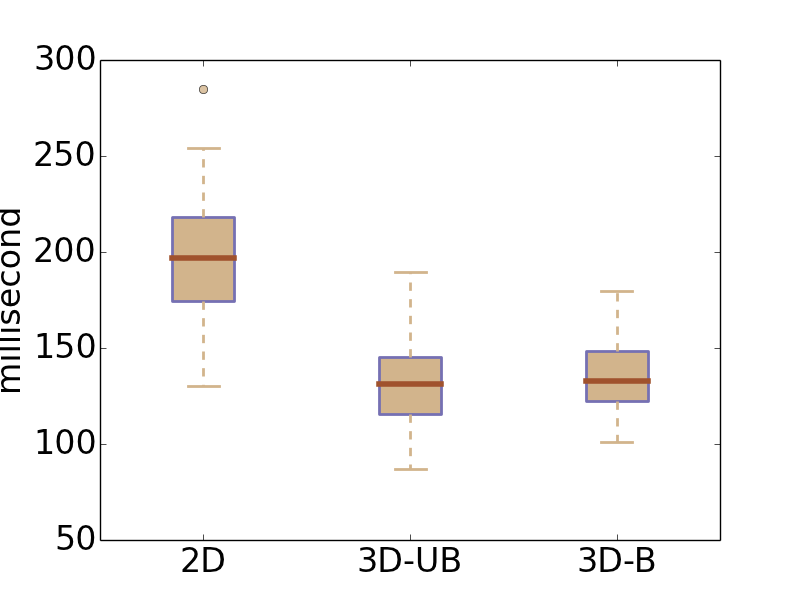
\includegraphics[height=1.5in]{figs/intra-job/shapestudy/cr_box}
        \caption{CrystalRouter}
        \label{fig:shapstudy-cr}
    \end{subfigure}%
    \begin{subfigure}[t]{0.32\textwidth}
        \centering
        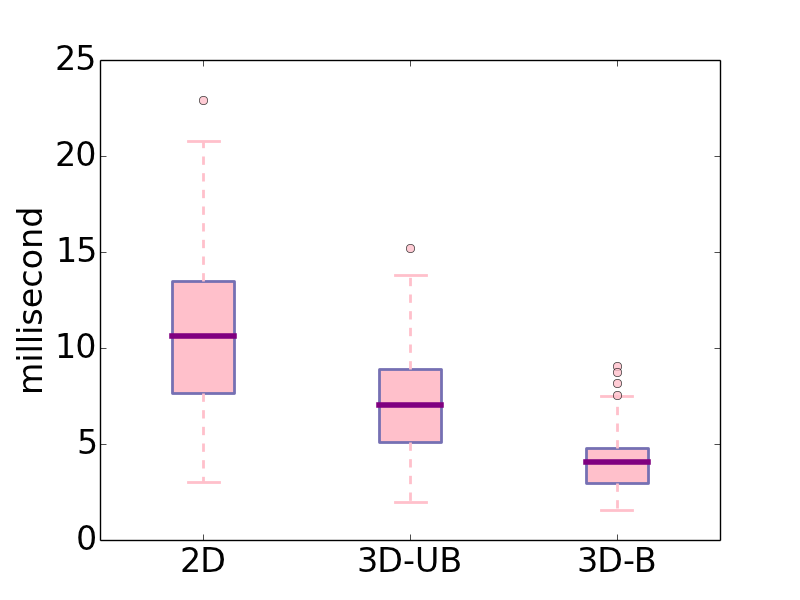
\includegraphics[height=1.5in]{figs/intra-job/shapestudy/mg_box}
        \caption{MultiGrid}
        \label{fig:shapstudy-mg}
    \end{subfigure}%
   \caption{Intra-job Study: Data Transfer Time of 3 Apps on 3 different shapes allocation}
   \label{fig: shapestudy}
\end{figure*}


In non-contiguous allocation systems, the nodes assigned to each job could be scatter anywhere in the system. Some HPC systems predefine the minimum number of nodes consist of the allocation unit. The nodes within each unit are contiguous, and units assigned to each job may have arbitrary locations. We assign each application with a non-contiguous set of allocation units, refers to a small number(like 4) of adjacent nodes as shown in Figure \ref{fig:noncont_sub1}. We compare application's performance when it runs with contiguous allocation and non-contiguous allocation with unit size of 16, as shown in Figure \ref{fig: cont-time-box}. 

Figure \ref{fig:cont-amg} shows that AMG is insensitive to the allocation's contiguity. Non-contiguous allocation can serve AMG equally well as contiguous allocation, as long as the allocation unit in non-contiguous allocation is big enough to preserve the locality of AMG. CrystalRouter shows preference in choosing between contiguous and non-contiguous allocation. As shown in Figure \ref{fig:cont-cr}, there is obvious degradation in terms data transfer time when CrystalRouter running with non-contiguous allocation. The global data transfer in CrystalRouter will take more hops on non-contiguous allocation, thus result in longer communication time. When it comes to MultiGrid shown in Figure \ref{fig:cont-mg}, this degradation is even worse. Since the global data transfer take a great portion of MultiGrid ``Many-to-Many" communication pattern. 

\emph{OBSERVATION}
The performance of application conforms to Nearest Neighbor communication pattern keep relatively stable with different allocations. Non-contiguous allocation won't aggravate intra-job interference as long as the unit size can preserve the locality in application's communication topology graph. 

\begin{figure*}[t!]
    \centering
    \begin{subfigure}[t]{0.32\textwidth}
        \centering
        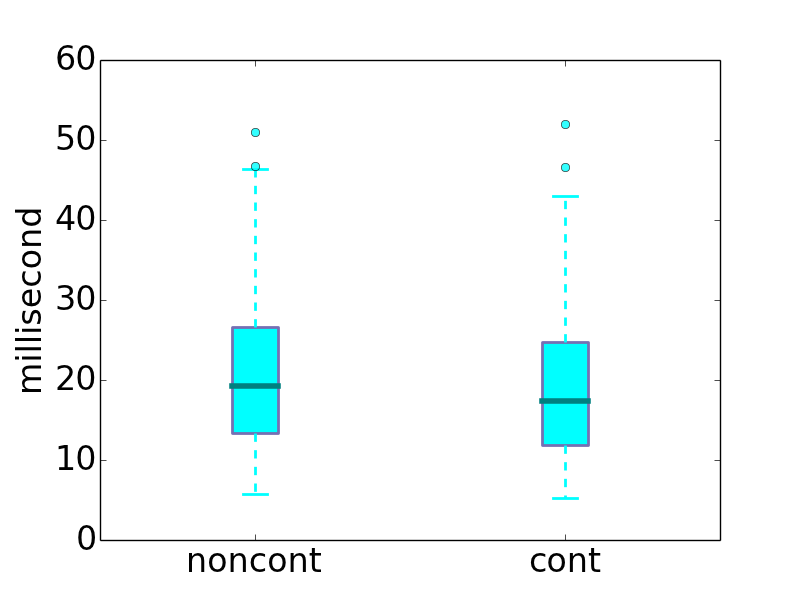
\includegraphics[height=1.5in]{figs/intra-job/cont/amg_box}
        \caption{AMG}
        \label{fig:cont-amg}
    \end{subfigure}%
    \hspace{1em}%
    \begin{subfigure}[t]{0.32\textwidth}
        \centering
        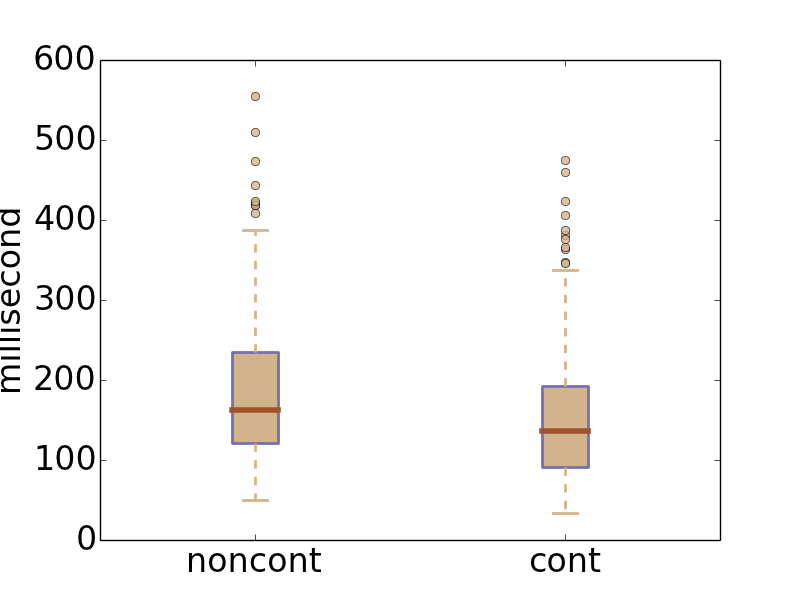
\includegraphics[height=1.5in]{figs/intra-job/cont/cr_box}
        \caption{CrystalRouter}
        \label{fig:cont-cr}
    \end{subfigure}%
    \begin{subfigure}[t]{0.32\textwidth}
        \centering
        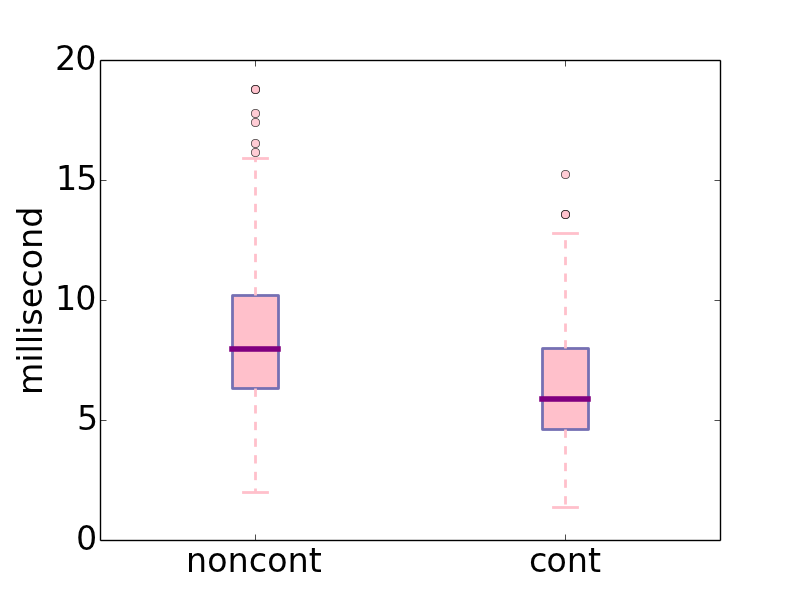
\includegraphics[height=1.5in]{figs/intra-job/cont/mg_box}
        \caption{MultiGrid}
        \label{fig:cont-mg}
    \end{subfigure}%
   \caption{Intra-job study: data transfer time of 3 apps with Non/Contiguous allocation}
   \label{fig: cont-time-box}
\end{figure*}

%Apparently, the size of allocation unit can affect application's performance. The good allocation unit size for each application is decided by application's communication pattern. Once the locality of application's communication pattern could be identified, the size of allocation unit should be able to preserve the locality of application. Figure \ref{fig: chunk-time-box} shows the data transfer time of 3 App with different allocation unit size. 
%
%For AMG, unit size of 16 and 8, are equally good, since AMG's locality is 6-rank based. Unit size of 2 can cause performance loss to AMG. For CrystalRouter data transfer time increases as the unit size decreases from 16 to 8 and 2. Unit size of 16 will preserve not only the 5-rank local community in CrystalRouter communication pattern, but also part of the diagonal global data transfer.  Unit size of 8 can only guarantee the locality of that 5-rank community. And unit size of 2 will lose all the locality of CrystalRouter and make the intra-job communication less efficient. For MultiGrid, smaller unit size prolong the data transfer time. The difference between different unit size is not obvious, since MultiGrid is nearly all-to-all dominant.
%
%
%\begin{figure*}[t!]
%    \centering
%    \begin{subfigure}[t]{0.3\textwidth}
%        \centering
%        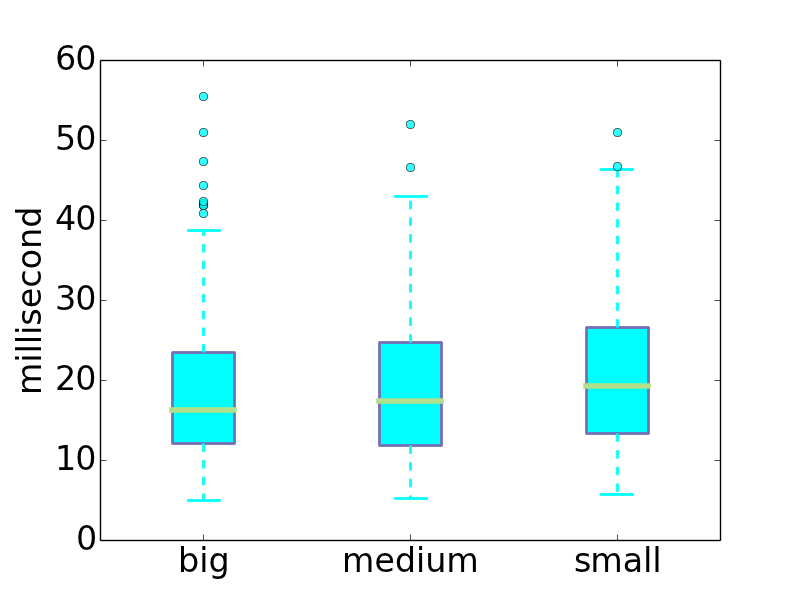
\includegraphics[height=1.2in]{figs/intra-job/chunk/amg_box}
%        \caption{AMG}
%        \label{fig:chunk-amg-box}
%    \end{subfigure}%
%    \hspace{1em}%
%    \begin{subfigure}[t]{0.3\textwidth}
%        \centering
%        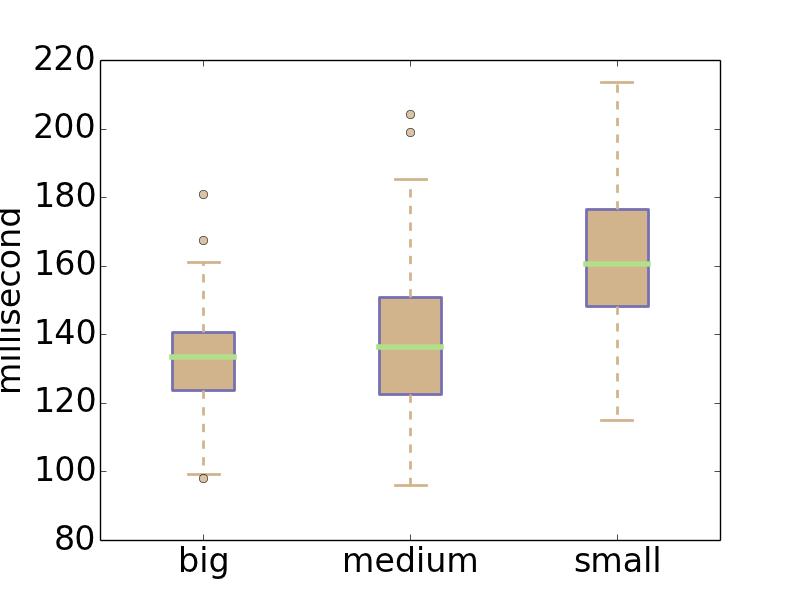
\includegraphics[height=1.2in]{figs/intra-job/chunk/cr_box}
%        \caption{CrystalRouter}
%        \label{fig:chunk-cr-box}
%    \end{subfigure}%
%    \hspace{1em}%
%    \begin{subfigure}[t]{0.3\textwidth}
%        \centering
%        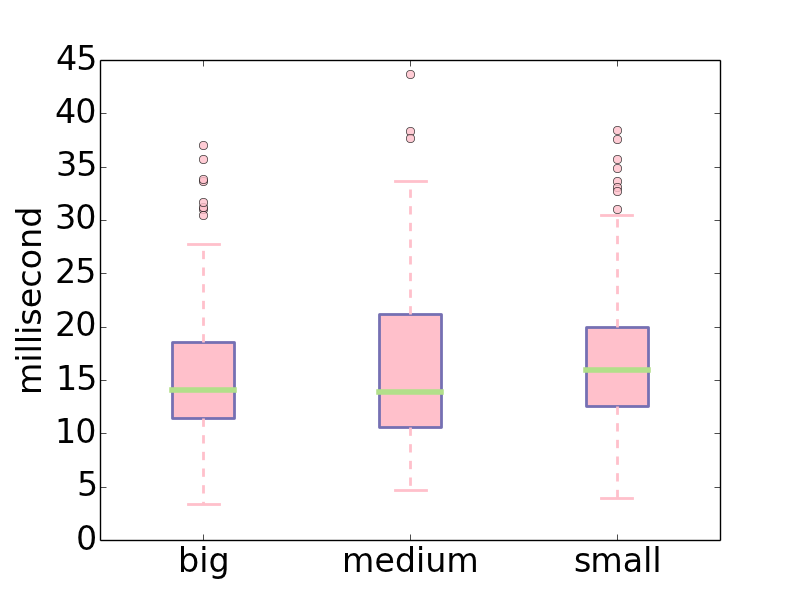
\includegraphics[height=1.2in]{figs/intra-job/chunk/mg_box}
%        \caption{MultiGrid}
%        \label{fig:chunk-mg-box}
%    \end{subfigure}%
%   \caption{Data Transfer Time of 3 Apps with Different Unit Size}
%   \label{fig: chunk-time-box}
%\end{figure*}




\subsubsection{Inter-Job Interference Analysis}
\label{sec: interjob interference study}

We simulate three application running concurrently with different allocation to analysis the interference between them. First, we assign each application with contiguous allocation side by side, and compare their performance with each application running exclusively. For AMG, sharing the network with other application won't affect its performance, since all the data transfer are between neighboring ranks. CrystalRouter and MultiGrid will suffer prolonged communication time when sharing network with others. The results are shown in Figure \ref{fig: concurrent-cont-time-box}.

Then, we assign each application with non-contiguous allocation and make them running concurrently. The allocation unit belongs to different jobs are interleaved as shown in Figure \ref{fig:noncont_sub1}. The unit size is critical to the application's performance. Figure \ref{fig: 3apps interjob study} shows the results of each application data transfer time with different allocation unit size. 

The data transfer time of AMG in Figure \ref{fig:interjob-amg-box} keeps stable between allocation unit size of 16(bit) and 8(medium), since the locality of AMG is 6-rank based. When the unit size reduce to 2(small), AMG suffers prolong data transfer time by about 10\%. CrystalRouter is more sensitive to allocation unit size. The best unit size would be the one big enough to accommodate its 5-rank locality. Figure \ref{fig:interjob-cr-box} shows unit size of 16 and 8 can guarantee the same average data transfer time, while some rank spend more time with allocation unit size 8 than 16. When the unit size reduce to 2-node, the communication become less efficiency and take 15\% more times for transferring data. 

The data transfer time of MultiGrid with different allocation unit sizes doesn't show obvious variability in Figure \ref{fig:interjob-mg-box}. This is because even big allocation unit size like 16 will still fail to preserve MultiGrid's ``Many-to-Many" pattern. The data transfer time is almost doubled when MultiGrid running concurrently with allocation unit size of 16, as shown in Figure \ref{fig:interjob-mg-box} . As the unit size decreases, the data transfer time keep growing, but in a slow way, which means in terms of preserving the locality of MultiGrid, allocation unit of size 16, 8 and 2 serve equally bad.

\emph{OBSERVATION}
The unit size in non-contiguous allocation policy should be chosen according to application's communication pattern. Inter-job interference is inevitable in non-contiguous based systems, but unit size that big enough to preserve the locality of the application will alleviate such interference and improve job performance. 



\begin{figure*}[t!]
    \centering
    \begin{subfigure}[t]{0.32\textwidth}
        \centering
        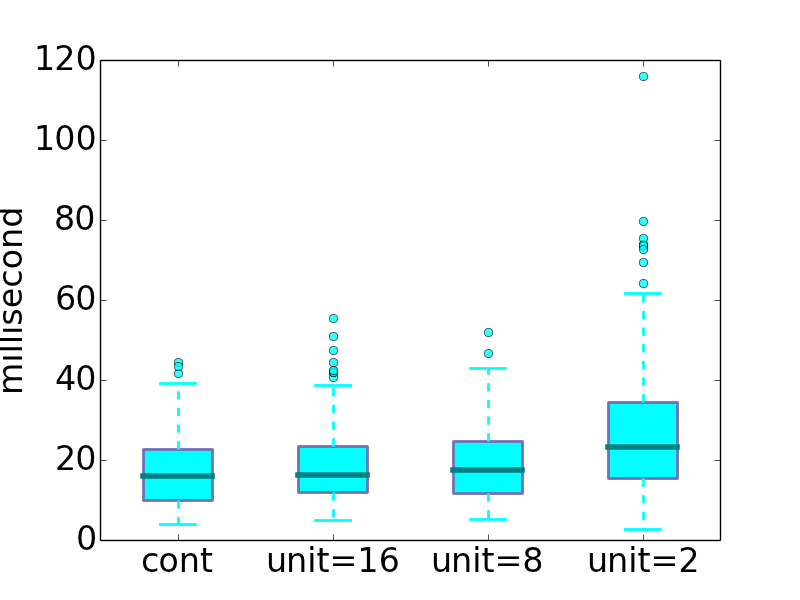
\includegraphics[height=1.5in]{figs/inter-job/amg}
        \caption{AMG}
        \label{fig:interjob-amg-box}
    \end{subfigure}%
    \hspace{1em}%
    \begin{subfigure}[t]{0.32\textwidth}
        \centering
        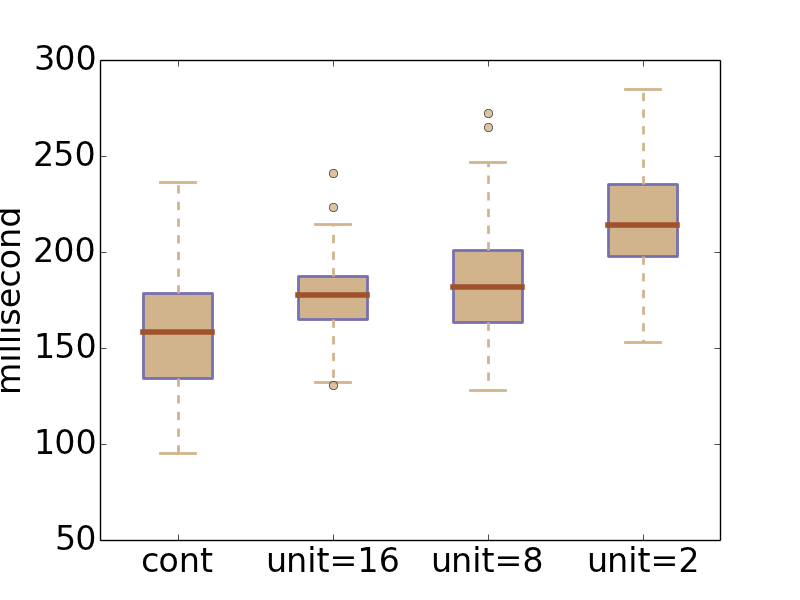
\includegraphics[height=1.5in]{figs/inter-job/cr}
        \caption{CrystalRouter}
        \label{fig:interjob-cr-box}
    \end{subfigure}%
    \begin{subfigure}[t]{0.32\textwidth}
        \centering
        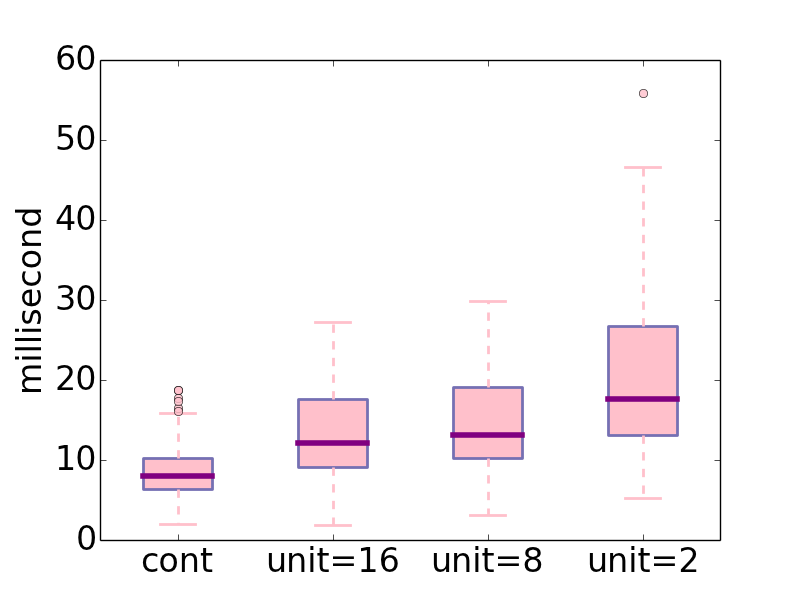
\includegraphics[height=1.5in]{figs/inter-job/mg}
        \caption{MultiGrid}
        \label{fig:interjob-mg-box}
    \end{subfigure}%
   \caption{Inter-job interference study. ``cont" indicates three applications running side by side concurrently on the same network with contiguous allocation. To study the impact of non-contiguous allocation, applications running concurrently with interleaved allocation of different unit sizes, which are 16-node, 8-node, 2-node. }
   \label{fig: 3apps interjob study}
\end{figure*}


\section{Discussion}
\label{sec:discussion}
HPC system usually accommodate many parallel jobs running concurrently. Each job gets the required number of computing nodes by system resource manager. The allocated nodes for each job communicate with each other through system interconnect network in a sharing way, which cause interference as a negative side-effect. This interference can introduce performance degradation to both job and system, such as prolonged job running time and reduced system throughput. 

The knowledge about HPC job's interference is extremely useful for improving system and job's performance. By scrutinizing job's communication behavior, we can locate the critical path with job's communication graph, identify  job's dominant communication pattern. With such knowledge about job's communication characteristics, we can analysis the possible interference between jobs through simulation or even predict such interference when job running on different allocations. 

The most promising way to utilize such knowledge is to make smart allocation based on job's dominant communication pattern. Most existing batch schedulers take so few initiative because it been hold under the obscurantism policy. Whether it use partition-based or non-contiguous policy, means it chooses the benefit of either system or job over the other. Some propose compromised policies \cite{lo}\cite{pascual}\cite{yang-cluster14} to use fix allocation unit size and  make the allocation for job blindly without knowing job's communication information. 

Based on the findings in this work, we propose the idea of smart job allocation with consideration about job's communication pattern. As the dominant communication pattern of parallel applications on HPC system can be summarized into a couple of categories, the deep understanding of one application can be helpful to all other applications that conforms to the same communication pattern. When an application with dominant communication that is intensive all-to-all submitted to the system, it should be granted with compact allocation with exclusive network provision, so that it won't suffer performance loss due to interference. If job with dominant communication pattern like Nearest Neighbor or others with intensive small scale communication, rather than assign it with unnecessary compact allocation and exclusive network provision, non-contiguous allocation with proper unit size would serve it equally well. No degradation will be introduced to job's performance and system utilization will be improved. 

The advantage of making allocation with consideration about job's communication pattern is obvious. First, compared with partition-based policy, the new allocation strategy is more flexible, it doesn't require the system to provide a big partition that can accommodate the whole application, just small set of compact nodes enough for all the "local community" in the application. On the other hand, the new allocation strategy won't destroy the locality of application's communication pattern. On the contrary, the small compact node set (allocation unit) provided for the application's  ``local communities"  will preserve the communication locality in the maximum extent.


%The off-line study of job's communication traces could be helpful to develop better allocation policies for batch scheduler to make on-line scheduling/allocating decisions. This is due to the set of applications running on those leadership computing facilities is usually stable, and the workloads from those HPC systems is usually has great repetitiveness. We analyzed the workload on Mira, an IBM Blue/Gene Q system at Argonne Leadership Computing Facility, found that a large portion of its workload are repetitive. Figure \ref{fig: repetitiveness of Mira} shows the 5 of most active users with repetitive submissions. The collected jobs information from history can be very useful for workload prediction and system optimization.
%
%
%\begin{figure}[h!] 
%  \centering
%  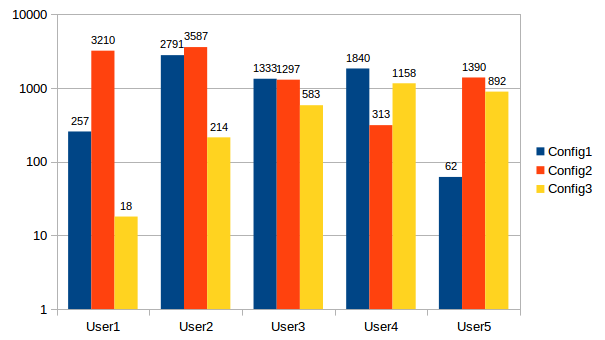
\includegraphics[width=0.38\textwidth]{figs/repe-mira}
%   \caption{The repetitiveness of Mira's workload. }
%   \label{fig: repetitiveness of Mira}
%\end{figure}




\section{Related Work}
\label{sec:related_work}
%\textbf{P1: tools for monitoring and profiling}\\
There are some tools available for system monitoring and application profiling on HPC systems. Tools like TAU (Tuning and Analysis) \cite{tau}, SCALASCA\cite{scala} and mpiP\cite{mpip} can capture application's runtime information about application's communication and computation in event traces. However, recognizing the patterns about application's communication from those traces requires lots of extra effort. Some researchers work on the recognition and characterization of parallel application communication patterns. Oak Ridge National Laboratory has this ongoing project about developing a tool set named Oxbow, which can characterize the computation and communication behavior of 12 scientific applications and benchmarks\cite{oxbow}. In their recent work\cite{hpdc2015-ornl}, they demonstrate a new approach to automatically characterizing a parallel application's communication behavior. 

%\textbf{P2: communication characteristics}\\
Some research institutes put great effort in characterization of scientific applications. The Department of Energy initiate this design forward project aims at the identification of the computational characteristics of the DOE MiniApps developed at various exascale co-design centers\cite{design forward webpage}. In this project, the communication patterns of several DOE full applications and associated mini-applications are studied to provide a more complete snapshot of the DOE workload. A joint project named CORAL from Oak Ridge, Argonne and Livermore provide a series of benchmarks to represent DOE workloads and technical requirements\cite{coral}. The CORAL project includes scalable science benchmarks, throughput benchmarks, data centric benchmarks, skeleton benchmarks and Micro benchmarks.  

%\textbf{P3: Interference between concurrently running jobs}\\
The interference between concurrently running jobs on HPC system have been identified as major culprit for job's performance variability. Abhinav et al. found that concurrently running applications on HPC can cause interference to each other, and cause communication time varied from 36\% faster to 69\% slower. Such interference could come from Operating System noise, shape of the allocated partition and mainly other running jobs that sharing network resources\cite{abhinav-sc13}. Skinner et al. found that  there is a 2-3$\texttimes$ slowdown in MPI$\textunderscore$Allreduce due to network contention from other jobs\cite{skinner}. Rosenthal et al. found there is limited benefit for many applications by increasing network bandwidth. The applications that send mostly small messages or larger messages asynchronously are not bandwidth bounded, hence, benefit only slightly or not at all from increased bandwidth\cite{rosenthal}.

%\textbf{P4: Job allocation(little bit)}\\
There are some research work focus on optimizing job allocation on HPC system to alleviate the interference between concurrently running jobs. Hoefler et al. propose to use performance modeling techniques to analysis factors that impact the performance of parallel scientific applications\cite{hoefler-modeling}. However, as the scale of HPC continue grows, the  interference of concurrently running jobs is getting worse, which is hard to be quantified by performance profiling tools. Bogdan et al provide a set of guidelines how to configure a network with Dragonfly topology for workload with Nearest Neighbor communication pattern\cite{Bogdan-hpdc14}. Dong et al describe IBM Blue Gene/Q's 5D torus interconnect network\cite{Dong-SC11}. They developed simple benchmarks that conforms to four different communication patterns, namely ping-pong, nearest neighbor, broadcast and allreduce, to demonstrate the effectiveness of this highly parallel 5D torus network.

Our work is different from all these works in the following ways. First, we focus on the dominant communication patterns rather than any specific application. We believe this can provide a guideline for other research work is the area. Secondly, we explored the inter-job interference between concurrently running jobs, while similar work such as \cite{abhinav-sc13} only focus on the single application's performance degradation due to network contention. Finally, we explored the impact of different allocation strategies to job's communication behavior. We identified the optimal allocation strategy for each application with specific dominant communication pattern. Based on our comprehensive exploration, we claim that better allocation strategy should take job's communication pattern into consideration for allocation decision making. 

\section{Conclusions}
\label{sec:conclusion}
In this work, we study the communication behavior of three parallel applications, namely AMG, CrystalRouter and MultiGrid. Each application has distinctive communication pattern, that can be representative for a group of jobs in HPC workload. We use a sophisticate simulation tool named CODES from Argonne National Laboratory to simulate the running of these three parallel applications on torus network. The torus network provided by CODES has good fidelity and scalability. We analyzed the performance of each application's communication in terms of data transfer time by simulating them running on torus networks with different bandwidth and dimensionality configurations. We found that higher dimensionality of torus network would improve the performance of application with ``Many-to-Many" communication patterns, while application with intensive local communication like ``Nearest Neighbor" won't benefit much from higher dimensionality.

We also analysis the intra- and inter-job interference by simulating three applications running on 3D torus network. Based on our comprehensive experiments, we got three observations. 1) The compact allocation can not guarantee the best performance for every application. 2) The performance of application conforms to Nearest Neighbor communication pattern keep relatively stable with different shape allocations, while application conforms to ``Many-to-Many" communication pattern prefer compact allocation. 3) The allocation unit size should be decided according to application's communication pattern. Unit size that big enough to preserve the locality of the application will result better performance. 

We believe that our finding in this work can provide guidance for HPC resource management to make flexible job allocations. Rather than use pre-defined partitions and reckless non-contiguous allocation, future HPC system should assign each job with preferable resources based on job's communication pattern. 

\section*{Acknowledgment}
\label{sec: ack}
The work at Illinois Institute of Technology is supported in part by U.S. National Science Foundation grants CNS-1320125 and CCF-1422009. This work is also supported by the U.S. Department of Energy, Office of Science, Advanced Scientific Computing Research, under Contract DE-AC02-06CH11357.


\begin{thebibliography}{10}
 %=====start of scheduling papers===== 

%\bibitem{yang-sc13}
%X. ~Yang, Z.~Zhou, S.~Wallace Z.~Lan, W.~Tang, S. ~Coghlan and Mike. ~Papka.
%\newblock Integrating Dynamic Pricing of Electricity into Energy Aware Scheduling for HPC Systems. 
%\newblock In {Proceedings of the International Conference on High Performance Computing, Networking, Storage and Analysis(SC), 2013 International Conference for}
%\newblock SC '13,
%\newblock 2013,
%\newblock Salt Lake City, Utah

%=====start of allocation aware papers===== 
\bibitem{leung}
V.J. Leung,  E.M. Arkin, M.A. Bender,  D. Bunde, J. Johnston, etc,
\newblock Processor allocation on Cplant: achieving general processor locality using one-dimensional allocation strategies
\newblock In {Proceedings of 2002 IEEE International Conference on Cluster Computing, 2002}.  pages 296--304, 2002

\bibitem{carl-cug}
Carl Albing and Mark Baker
\newblock ALPS,Topology, and Performance: A Comparison of Linear Orderings for 
Application Placement in a 3D torus.
\newblock Presented at the CUG 2010, Edinburgh, Scotland, UK, 2010.

\bibitem{yang-cluster14}
Xu Yang and Zhou Zhou and Wei Tang and Xingwu Zheng and Jia Wang and Zhiling Lan.
\newblock Cluster Computing (CLUSTER), 2014 IEEE International Conference on,
\newblock Balancing job performance with system performance via locality-aware scheduling on torus-connected systems
\newblock Sept, 2014,
\newblock pp.140-148

\bibitem{lo}
V. Lo,  K. Windisch, W.  Liu, and Nitzberg.
\newblock Noncontiguous processor allocation algorithms for mesh-connected multicomputers.
\newblock IEEE Transactions on Parallel and Distributed Systems 8 (1997). pages 712--726

\bibitem{pascual} 
JA. Pascual, J. Navaridas and  J. Miguel-Alonso. 
\newblock Effects of Topology-Aware Allocation Policies on Scheduling Performance. 
\newblock 14th Workshop on Job Scheduling Strategies for Parallel Processing. May 29, 2009.Rome, Italy.


%+++++++++++++++++++++++
\bibitem{mpip}
\newblock mpiP: Lightweight, Scalable MPI Profiling.
\newblock http://mpip.sourceforge.net, 
\newblock 2013.

\bibitem{tau}
S. Shende and A. Malony. 
\newblock The TAU parallel performance system. 
\newblock International Journal of High Performance Computing Applications, 20(2):287–311, 2006.

\bibitem{scala}
X. Wu, F. Mueller, S. Pakin, 
\newblock "Automatic Generation of Executable Communication Specifications from Parallel Applications", 
\newblock In {Proceedings of the International Conference on High Performance Computing, Networking, Storage and Analysis(SC), 2011 International Conference for}
\newblock SC '11,
\newblock 2011,pages 12-21.

\bibitem{design forward webpage}
Department of Energy, “Characterization of the DOE Mini-apps.” [Online].
\newblock Available: http://portal.nersc.gov/project/CAL/trace.htm
\newblock (Accessed on: Sept 16th. 2015)


\bibitem{coral}
CORAL collaboration benchmark codes [Online].
\newblock Available:https://asc.llnl.gov/CORAL-benchmarks/
\newblock (Accessed on: Sept 16th. 2015)

\bibitem{ipm}
David Skinner, Nicholas Wright, Karl Fuerlinger and Kathy Yelick
\newblock Integrated Performance Montoring(IPM)
\newblock Available http://ipm-hpc.sourceforge.net/overview.html
\newblock (Accessed on: Sept 16th. 2015)


\bibitem{miniapp}
Bronson Messer
\newblock "Using a Developing MiniApp to Compare Platform Characteristics on Cray Systems"
\newblock In Proceedings of Cray User Group 2012

\bibitem{amg}
V. E. Henson and U. M. Yang, 
\newblock "BoomerAMG: A Parallel Algebraic Multigrid Solver and Preconditioner",
\newblock Appl. Num. Math. 41 (2002), pp. 155-177. UCRL-JC-141495.

\bibitem{crystalrouter}
P. Fischer, J. Lottes, D. Pointer, and A. Siegel, 
\newblock “Petascale algorithms for reactor hydrodynamics,”
\newblock Journal of Physics: Conference Series, vol. 125, no. 1, p. 012076, 2008.

%+++++++++++++++++

%=====start of network papers===== 
\bibitem{rosenthal}
E. Rosenthal and E.A. Leon
\newblock Characterizing Application Sensitivity to Network Performance.
\newblock  In {Proceedings of SC14: International
Conference for High Performance Computing, Networking, Storage and Analysis},
2014

\bibitem{hoefler-modeling}
T. Hoefler and W. Gropp and M. Snir and W. Kramer
\newblock Performance Modeling for Systematic Performance Tuning,
\newblock 2011
\newblock Nov.
\newblock In {Proceedings of International Conference for High Performance Computing, Networking, Storage and Analysis (SC'11), SotP Session,
}

\bibitem{roth}
P. Roth and J. Meredith and J. Vetter,
\newblock "Automated Characterization of Parallel Application Communication Patterns",
In Proceedings of the 25rd International Symposium on High-performance Parallel and Distributed Computing
\newblock HPDC '15,
\newblock 2015,


%=====end of application/mapping papers===== 

\bibitem{RF}
Fiedler, Robert, and Stephen Whalen. 
\newblock "Improving task placement for applications with 2D, 3D, and 4D virtual Cartesian topologies on 3D torus networks with service nodes." 
\newblock Proc. Cray User’s Group (2013).



\bibitem{abhinav-sc13} 
Bhatele, Abhinav and Mohror, Kathryn and Langer, Steven
H. and Isaacs, Katherine E. 
\newblock There Goes the Neighborhood: Performance Degradation Due to Nearby Jobs 
\newblock In {Proceedings of SC13: International
Conference for High Performance Computing, Networking, Storage and Analysis},
2013

\bibitem{jose-ipdps15}
Jokanovic, A.; Sancho, J.C.; Rodriguez, G.; Lucero, A.; Minkenberg, C.; Labarta, J.,
\newblock "Quiet Neighborhoods: Key to Protect Job Performance Predictability," 
\newblock in Parallel and Distributed Processing Symposium (IPDPS), 
\newblock 2015 IEEE International , vol., no., pp.449-459, 25-29 May 2015

\bibitem{skinner}
D. Skinner and W. Kramer. 
\newblock Understanding the Causes of Performance Variability in HPC Workloads. 
\newblock In Proceedings of the IEEE International Workload Characterization Symposium, 
\newblock 2005, pages 137–149, 2005.

\bibitem{hpdc14}
Prisacari, Bogdan and Rodriguez, German and Heidelberger, Philip and Chen, Dong and Minkenberg, Cyriel and Hoefler, Torsten
\newblock Efficient Task Placement and Routing of Nearest Neighbor Exchanges in Dragonfly Networks
\newblock In Proceedings of the 23rd International Symposium on High-performance Parallel and Distributed Computing
\newblock HPDC '14,
\newblock 2014,
\newblock Vancouver, BC, Canada

\bibitem{jingjin}
Wu, Jingjin and Lan, Zhiling and Xiong, Xuanxing and Gnedin, Nickolay Y. and Kravtsov, Andrey V.
\newblock Hierarchical Task Mapping of Cell-based AMR Cosmology Simulations
\newblock Proceedings of the International Conference on High Performance Computing, Networking, Storage and Analysis
\newblock SC '12,
\newblock 2012,
\newblock Salt Lake City, Utah

\bibitem{ozan}
Tuncer, Ozan, Vitus J Leung, Ayse K. Coskun,
\newblock "PaCMap: Topology Mapping of Unstructured Communication Patterns onto Non-contiguous Allocations," 
\newblock 29th International Conference on Supercomputing, June 2015.


\bibitem{zhou-ipdps}
Z. Zhou, X. Yang, Z. Lan, P. Rich, W. Tang, V. Morozov, and N. Desai.
\newblock Improving Batch Scheduling on Blue Gene/Q by Relaxing 5D Torus Network Allocation Constraints,
\newblock Proceedings of 29th IEEE International Parallel \& Distributed Processing 
Symposium,
\newblock IPDPS'15, 2015.
\newblock Hyderabad, INDIA

\bibitem{Bogdan-hpdc14}
Prisacari, Bogdan and Rodriguez, German and Heidelberger, Philip and Chen, Dong and Minkenberg, Cyriel and Hoefler, Torsten
\newblock Efficient Task Placement and Routing of Nearest Neighbor Exchanges in Dragonfly Networks,
\newblock Proceedings of the 23rd International Symposium on High-performance Parallel and Distributed Computing,
\newblock HPDC '14,
\newblock 2014,
\newblock  Vancouver, BC, Canada,


\bibitem{hpdc2015-ornl}
Philip. C.R, Jeremy S. M, etc
\newblock "Automated Characterization of Parallel Application Communication Patterns"
\newblock HPDC'15

\bibitem{oxbow}
J. S. Vetter, S. Lee, D. Li, G. Marin, C. McCurdy, J. Meredith, P. C. Roth, and K. Spafford. 
\newblock Quantifying architectural requirements of contemporary extreme-scale scientific applications. 
\newblock In International Workshop on Performance Modeling, Benchmarking and Simulation of HPC Systems (PMBS13), 
\newblock Denver, Colorado, 2013.

\bibitem{Dong-SC11}
Dong Chen; Eisley, N.A.; Heidelberger, P.; Senger, R.M.; Sugawara, Y.; Kumar,
S.; Salapura, V.; Satterfield, D.L.; Steinmacher-Burow, B.; Parker, J.J., 
\newblock "The IBM Blue Gene/Q interconnection network and message unit," 
\newblock High Performance Computing, Networking, Storage and Analysis (SC), 2011 International 
Conference,
\newblock pp.1,10, 
\newblock 12-18 Nov. 2011

\bibitem{Jason-2011}
Jason Cope, Ning Liu, Sam Lang, Phil Carns, Chris Carothers, Robert Ross.
\newblock CODES: Enabling Co-design of Multilayer Exascale Storage Architectures, 
\newblock Proceedings of the Workshop on Emerging Supercomputing Technologies 2011, pp. 303-312
\newblock 2011


%===simulation papers =====

\bibitem{ross}
P. D. Barnes, C. D. Carothers, D. R. Jefferson, and J. M. LaPre, 
\newblock “Warp speed: executing time warp on 1,966,080 cores,”
\newblock in Proc. of the 2013 ACM SIGSIM Conf. on Principles of Advanced Discrete Simulation (PADS),
\newblock May 2013, pp. 327–336.

\bibitem{mubarak-sc2012}
Mubarak, M.; Carothers, C.D.; Ross, R.; Carns, P.,
\newblock "Modeling a Million-Node Dragonfly Network Using Massively Parallel Discrete-Event Simulation," 
\newblock High Performance Computing, Networking, Storage and Analysis (SCC), 
\newblock 2012 SC Companion: 
\newblock pp.366,376, 10-16 Nov. 2012

\bibitem{codes-torus}
Mubarak, Misbah, et al.
\newblock "A case study in using massively parallel simulation for extreme-scale torus network codesign." 
\newblock in Proceedings of the 2nd ACM SIGSIM/PADS conference on Principles of advanced discrete simulation. 
\newblock ACM, 2014.

\bibitem{bgq}
C. Dong, N. Eisley, P. Heidelberger, R. Senger, Y. Sugawara, S. Kumar, V. Salapura, D. Satterfield, B. Steinmacher-Burow, and J. Parker, 
\newblock “The IBM Blue Gene/Q interconnection fabric,” 
\newblock Micro, IEEE, vol. 32, no. 1, pp. 32–43, 2012.

\bibitem{tofu}
Y. Ajima, Y. Takagi, T. Inoue, S. Hiramoto, and T. Shimizu, 
\newblock “The Tofu Interconnect,” 
\newblock in 2011 IEEE 19th Annual Symposium on High Performance Interconnects (HOTI), 2011, pp. 87–94.

\bibitem{titan}
Titan System Overview [online]
\newblock Available: https://www.olcf.ornl.gov/kbarticles/titan-system-overview
\newblock (Accessed on: OCT 4th, 2015)


\bibitem{sst}
Sandia National Labs, “SST DUMPI trace library.” [Online].
\newblock Available: http://sst.sandia.gov/using dumpi.html 
\newblock (Accessed on: Sept 3rd, 2015)

\bibitem{simgrid}
SIMGRID Versatile Simulation of Distributed Systems [Online].
\newblock Availabale: http://simgrid.gforge.inria.fr
\newblock (Accessed on: Oct 4th, 2015)

\bibitem{top500}
“Top500 supercomputing web site.” [Online]. 
\newblock Available: http://www.top500.org
\newblock (Accessed on: Oct 4th, 2015)


\end{thebibliography}


\vspace{5\baselineskip}
The submitted manuscript has been created by UChicago Argonne, LLC, Operator of Argonne National Laboratory ("Argonne").  Argonne, a U.S. Department of Energy Office of Science laboratory, is operated under Contract No. DE-AC02-06CH11357.  The U.S. Government retains for itself, and others acting on its behalf, a paid-up nonexclusive, irrevocable worldwide license in said article to reproduce, prepare derivative works, distribute copies to the public, and perform publicly and display publicly, by or on behalf of the Government.


\end{document}


